\documentclass[11pt]{article}

\usepackage[a4paper,margin=0.75in]{geometry}
\usepackage[T1]{fontenc}
\usepackage[utf8]{inputenc}
\usepackage{lmodern}
\usepackage{xcolor}
\usepackage{amsmath,amssymb,amsthm,mathtools,bm}
\usepackage{enumitem}
\usepackage{booktabs}
\usepackage{array}
\usepackage{longtable}
\usepackage{pdflscape}
\usepackage{graphicx}
\usepackage{tikz}
\usetikzlibrary{arrows.meta}
\usepackage{hyperref}
\usepackage{float}
\usepackage{multirow}

\hypersetup{
  colorlinks=true,
  hypertexnames=false,
  linkcolor=blue!50!black,
  citecolor=blue!50!black,
  urlcolor=blue!50!black
}

% To do macro
\newcommand{\todo}[1]{\textcolor{red}{#1}}

% Blackboard bold macros
\newcommand{\dsA}{\mathbb{A}}
\newcommand{\dsB}{\mathbb{B}}
\newcommand{\dsC}{\mathbb{C}}
\newcommand{\dsD}{\mathbb{D}}
\newcommand{\dsE}{\mathbb{E}}
\newcommand{\dsF}{\mathbb{F}}
\newcommand{\dsG}{\mathbb{G}}
\newcommand{\dsH}{\mathbb{H}}
\newcommand{\dsI}{\mathbb{I}}
\newcommand{\dsJ}{\mathbb{J}}
\newcommand{\dsK}{\mathbb{K}}
\newcommand{\dsL}{\mathbb{L}}
\newcommand{\dsM}{\mathbb{M}}
\newcommand{\dsN}{\mathbb{N}}
\newcommand{\dsO}{\mathbb{O}}
\newcommand{\dsP}{\mathbb{P}}
\newcommand{\dsQ}{\mathbb{Q}}
\newcommand{\dsR}{\mathbb{R}}
\newcommand{\dsT}{\mathbb{T}}
\newcommand{\dsU}{\mathbb{U}}
\newcommand{\dsV}{\mathbb{V}}
\newcommand{\dsW}{\mathbb{W}}
\newcommand{\dsX}{\mathbb{X}}
\newcommand{\dsY}{\mathbb{Y}}
\newcommand{\dsZ}{\mathbb{Z}}

% Calligraphic macros
\newcommand{\scA}{\mathcal{A}}
\newcommand{\scB}{\mathcal{B}}
\newcommand{\scC}{\mathcal{C}}
\newcommand{\scD}{\mathcal{D}}
\newcommand{\scE}{\mathcal{E}}
\newcommand{\scF}{\mathcal{F}}
\newcommand{\scG}{\mathcal{G}}
\newcommand{\scH}{\mathcal{H}}
\newcommand{\scI}{\mathcal{I}}
\newcommand{\scJ}{\mathcal{J}}
\newcommand{\scK}{\mathcal{K}}
\newcommand{\scL}{\mathcal{L}}
\newcommand{\scM}{\mathcal{M}}
\newcommand{\scN}{\mathcal{N}}
\newcommand{\scO}{\mathcal{O}}
\newcommand{\scP}{\mathcal{P}}
\newcommand{\scQ}{\mathcal{Q}}
\newcommand{\scR}{\mathcal{R}}
\newcommand{\scS}{\mathcal{S}}
\newcommand{\scT}{\mathcal{T}}
\newcommand{\scU}{\mathcal{U}}
\newcommand{\scV}{\mathcal{V}}
\newcommand{\scW}{\mathcal{W}}
\newcommand{\scX}{\mathcal{X}}
\newcommand{\scY}{\mathcal{Y}}
\newcommand{\scZ}{\mathcal{Z}}

\newcommand{\HomG}[2]{\operatorname{Hom}_G\!\left(#1,#2\right)}
\newcommand{\Sym}{\operatorname{Sym}}
\newcommand{\Span}{\operatorname{span}}
\newcommand{\mult}{\operatorname{mult}}
\newcommand{\ev}{\operatorname{ev}}
\newcommand{\id}{\operatorname{id}}
\newcommand{\GL}{\operatorname{GL}}
\newcommand{\SO}{\operatorname{SO}}
\newcommand{\Orth}{\operatorname{O}}
\newcommand{\diag}{\operatorname{diag}}
\newcommand{\tr}{\operatorname{tr}}
\newcommand{\wt}{\operatorname{wt}}
\newcommand{\SSYT}{\operatorname{SSYT}}
\newcommand{\set}[1]{\{#1\}}
\newcommand{\TTempty}{\ensuremath{\dsI}}
\newcommand{\TT}[1]{\langle #1\rangle}
\tikzset{
  ttdot/.style={circle, fill=black, inner sep=0pt, minimum size=2.2pt},
  ttwire/.style={line width=0.45pt},
  ttlabel/.style={inner sep=0.5pt}
}
\newcommand{\TTid}{\ensuremath{\dsI}}
\newcommand{\TTbin}[3]{%
  \begin{tikzpicture}[baseline=-0.5ex,x=1.05em,y=1.05em]
    \node[ttdot] (v) at (0,0) {};
    \draw[ttwire] (-1,0) -- (v) node[pos=0.45,above,ttlabel] {$#1$};
    \draw[ttwire] (v) -- (1,0) node[pos=0.55,above,ttlabel] {$#3$};
    \draw[ttwire] (v) -- (0,-0.82) node[pos=0.85,right,ttlabel] {$#2$};
  \end{tikzpicture}%
}
\newcommand{\TTtwo}[5]{%
  \begin{tikzpicture}[baseline=-0.5ex,x=0.95em,y=0.95em]
    \node[ttdot] (a) at (-0.55,0) {};
    \node[ttdot] (b) at (0.85,0) {};
    \draw[ttwire] (-1.55,0) -- (a) node[pos=0.45,above,ttlabel] {$#1$};
    \draw[ttwire] (a) -- (b) node[midway,above,ttlabel] {$#3$};
    \draw[ttwire] (b) -- (1.85,0) node[pos=0.55,above,ttlabel] {$#5$};
    \draw[ttwire] (a) -- (-0.55,-0.82) node[pos=0.85,right,ttlabel] {$#2$};
    \draw[ttwire] (b) -- (0.85,-0.82) node[pos=0.85,right,ttlabel] {$#4$};
  \end{tikzpicture}%
}
\newcommand{\TTcolbin}[3]{%
  \begin{tikzpicture}[baseline=-0.5ex,x=1.05em,y=1.05em]
    \node[ttdot] (v) at (0,0) {};
    \draw[ttwire] (-1,0) -- (v) node[pos=0.45,above,ttlabel] {$#1$};
    \draw[ttwire] (v) -- (1,0) node[pos=0.55,above,ttlabel] {$#3$};
    \draw[ttwire] (v) -- (0,-0.82) node[pos=0.85,right,ttlabel] {$#2$};
  \end{tikzpicture}%
}
\newcommand{\TThooktree}[5]{%
  \begin{tikzpicture}[baseline=-0.5ex,x=0.95em,y=0.95em]
    \node[ttdot] (c) at (-0.8,0) {};
    \node[ttdot] (i) at (0.7,0) {};
    \draw[ttwire] (-1.75,0) -- (c) node[pos=0.45,above,ttlabel] {$#1$};
    \draw[ttwire] (c) -- (i) node[midway,above,ttlabel] {$#3$};
    \draw[ttwire] (i) -- (1.65,0) node[pos=0.55,above,ttlabel] {$#5$};
    \draw[ttwire] (c) -- (-0.8,-0.82) node[pos=0.85,right,ttlabel] {$#2$};
    \draw[ttwire] (i) -- (0.7,-0.82) node[pos=0.85,right,ttlabel] {$#4$};
  \end{tikzpicture}%
}
\tikzset{youngcell/.style={draw, minimum size=1.35em, inner sep=0pt}}
\newcommand{\Ybox}[3]{\node[youngcell] at (#1,#2) {\scriptsize $#3$};}
\newcommand{\Yempty}{\ensuremath{\varnothing}}
\newcommand{\Yone}[1]{%
  \begin{tikzpicture}[baseline=-0.55ex,x=1.35em,y=1.35em]
    \Ybox{0}{0}{#1}
  \end{tikzpicture}%
}
\newcommand{\Yrowtwo}[2]{%
  \begin{tikzpicture}[baseline=-0.55ex,x=1.35em,y=1.35em]
    \Ybox{0}{0}{#1}
    \Ybox{1}{0}{#2}
  \end{tikzpicture}%
}
\newcommand{\Yrowthree}[3]{%
  \begin{tikzpicture}[baseline=-0.55ex,x=1.35em,y=1.35em]
    \Ybox{0}{0}{#1}
    \Ybox{1}{0}{#2}
    \Ybox{2}{0}{#3}
  \end{tikzpicture}%
}
\newcommand{\Ycoltwo}[2]{%
  \begin{tikzpicture}[baseline=-0.2ex,x=1.35em,y=1.35em]
    \Ybox{0}{0}{#1}
    \Ybox{0}{-1}{#2}
  \end{tikzpicture}%
}
\newcommand{\Yhook}[3]{%
  \begin{tikzpicture}[baseline=-0.2ex,x=1.35em,y=1.35em]
    \Ybox{0}{0}{#1}
    \Ybox{1}{0}{#2}
    \Ybox{0}{-1}{#3}
  \end{tikzpicture}%
}
\newcommand{\YDset}[1]{\ensuremath{\left\{\vcenter{\hbox{#1}}\right\}}}
\newcommand{\LeafTensorPair}[2]{%
  \begin{tabular}{@{}c@{}}#1\\[0.05em]#2\end{tabular}%
}
\newcommand{\IsoLeafData}[7]{%
  \begingroup
  \renewcommand{\arraystretch}{1.1}%
  \begin{tabular}{@{}c@{}}
    $\boldsymbol{\mu}=#1\quad \#=#7$\\[0.05em]
    \begin{tabular}{@{}c@{\hspace{0.65em}}c@{\hspace{0.65em}}c@{}}
      $C$ & $L_2,T_2$ & $L_3,T_3$\\[0.05em]
      #2 & \LeafTensorPair{#3}{#4} & \LeafTensorPair{#5}{#6}
    \end{tabular}
  \end{tabular}%
  \endgroup
}
\newcommand{\IsoTensorData}[5]{%
  \begingroup
  \renewcommand{\arraystretch}{1.1}%
  \setlength{\tabcolsep}{1.7pt}%
  \begin{tabular}{@{}c@{\hspace{0.35em}}c@{\hspace{0.35em}}c@{\hspace{0.35em}}c@{\hspace{0.35em}}c@{}}
    $C$ & $L_2$ & $T_2$ & $L_3$ & $T_3$\\[0.05em]
    #1 & #2 & #3 & #4 & #5
  \end{tabular}%
  \endgroup
}

\newtheorem{theorem}{Theorem}[section]
\newtheorem{proposition}[theorem]{Proposition}
\newtheorem{lemma}[theorem]{Lemma}
\newtheorem{corollary}[theorem]{Corollary}
\newtheorem{algorithm}[theorem]{Algorithm}
\newtheorem{assumption}{Assumption}[section]

\theoremstyle{definition}
\newtheorem{definition}[theorem]{Definition}
\newtheorem{example}[theorem]{Example}
\newtheorem{remark}[theorem]{Remark}

\title{Equivariant Learning via Minimal Integrity Bases for Equivariant Polynomials}
\author{Michael Liaofan Liu}
\date{}

\begin{document}
\maketitle

\begin{abstract}

  We present a general framework for equivariant learning when the underlying group is linearly reductive.
  Our approach enforces equivariance by a one-time computation of minimal integrity bases for the covariant module and invariant algebra of equivariant and invariant polynomials.
  In particular, the trainable parameters in our model lie entirely in an unconstrained neural network whose architecture can be chosen arbitrarily.
  Moreover, if untruncated integrity bases are used, our hypothesis class is dense in the space of continuous equivariant functions with the sup norm.
  To compute minimal integrity bases, we first enumerate vector space bases for the covariant module and invariant algebra as candidate generators.
  Then, we apply the graded Nakayama lemma to extract independent generators degree by degree.
  We implement our algorithms in full generality: given explicit isotypic decompositions for the input and output representations, as well as explicit Clebsch--Gordan decompositions for the tensor product of irreducible representations, our algorithms work for any linearly reductive group.
  In particular, we provide end-to-end implementations for the groups $\SO(2)$, $\SO(3)$, $\Orth(2)$, and $\Orth(3)$. We also discuss how to enforce translation and permutation equivariance within our framework.
  Our code is available on GitHub at \href{https://github.com/MichaelLiu2024/Equivariant-Polynomial-Tensor-Functions}{\texttt{github.com/MichaelLiu2024/Equivariant-Polynomial-Tensor-Functions}}.

\end{abstract}

\section{Introduction}

%A central problem in supervised equivariant machine learning is to learn an unknown equivariant function given a dataset of input-output pairs.
%To solve this problem, many existing equivariant neural network architectures enforce equivariance via layerwise constraints.
%While layerwise architectures have been successfully applied in a variety of settings, they have a number of shortcomings.
%For instance, the choice of hidden representations is arbitrary and can contribute to undesirable scaling in the number of trainable parameters: substantial parameter budget may be spent learning equivariant maps between hidden representations.
%Ordinary pointwise nonlinearities are compatible in settings such as G-CNN feature fields~\cite{cohen2016gcnn}, but for general representation-valued features, gated, norm-based, or tensor-product nonlinearities are often required to ensure equivariance~\cite{finzi2021emlp, Thomas2018tfn, kondor2018cgnets}.
%In particular, tensor-product nonlinearities can create large quadratic expansions before compression.

Let $X$ and $Y$ be finite-dimensional complex representations of a linearly reductive group $G$.
Let $F\colon X\to Y$ be an unknown $G$-equivariant function which we wish to learn.
To begin, suppose that $F$ is a polynomial.
Then $F$ lies in the \emph{covariant module}
\[
  \scM_G(X,Y)\coloneq\left(\scS(X^*)\otimes Y\right)^G
\]
of $G$-equivariant polynomials from $X$ to $Y$.
This is a module over the \emph{invariant algebra}
\[
  \scR_G(X)\coloneq\scS(X^*)^G
\]
of $G$-invariant polynomials on $X$.
Now, suppose that we can compute minimal $\scR_G(X)$-module generators $\set{m_1,\dots,m_M}\subseteq \scM_G(X,Y)$ and minimal $\dsC$-algebra generators $\set{r_1,\dots,r_R}\subseteq \scR_G(X)$.
Then $F$ admits a decomposition
\begin{equation}\label{eq:polynomial-ansatz}
  F(x)=\sum_{i=1}^M p_{\theta,i}(r_1(x),\dots,r_R(x))m_i(x),
\end{equation}
where $p_\theta\colon \dsC^R\to\dsC^M$ is some polynomial with coefficients $\theta$.
Thus, learning $F$ reduces to learning $\theta$.

Now, suppose that $F$ is merely continuous.
Replacing the polynomial $p_\theta$ above with a neural network $\scN_\theta\colon \dsC^R\to\dsC^M$, we obtain a large class of $G$-equivariant functions
\begin{equation}\label{eq:neural-ansatz}
  F_\theta(x)=\sum_{i=1}^M
  \scN_{\theta,i}(r_1(x),\dots,r_R(x))m_i(x),
\end{equation}
and it remains only to learn $\theta$ so that $F_\theta \approx F$. We note that special cases of the ansatz in Eq.~\eqref{eq:neural-ansatz} have appeared before in the literature \cite{BlumSmithVillar2023}.

Some remarks on the properties of our ansatz in Eq.~\eqref{eq:neural-ansatz}:
\begin{itemize}
  \item equivariance follows automatically since the $m_i$ are equivariant and the $r_j$ are invariant;
  \item as a result, the neural network $\scN_\theta$ may have any standard architecture and any standard nonlinearities with no additional equivariance constraints;
  \item assuming that the neural network class $\set{\scN_\theta}_{\theta}$ is sufficiently expressive, our ansatz can approximate any continuous $G$-equivariant function $F$ arbitrarily well in the sup norm (see Theorem \ref{thm:universal-approximation});
  \item for fixed $(G,X,Y)$, the one-time computation of the generators $\set{m_1,\dots,m_M}$ and $\set{r_1,\dots,r_R}$ can be reused to learn multiple $G$-equivariant functions $F_1, F_2, \ldots$ from $X$ to $Y$ by training different neural networks $\scN_{\theta_1}, \scN_{\theta_2}, \ldots$.
\end{itemize}


\begin{figure}[H]
\centering
\resizebox{0.98\textwidth}{!}{%
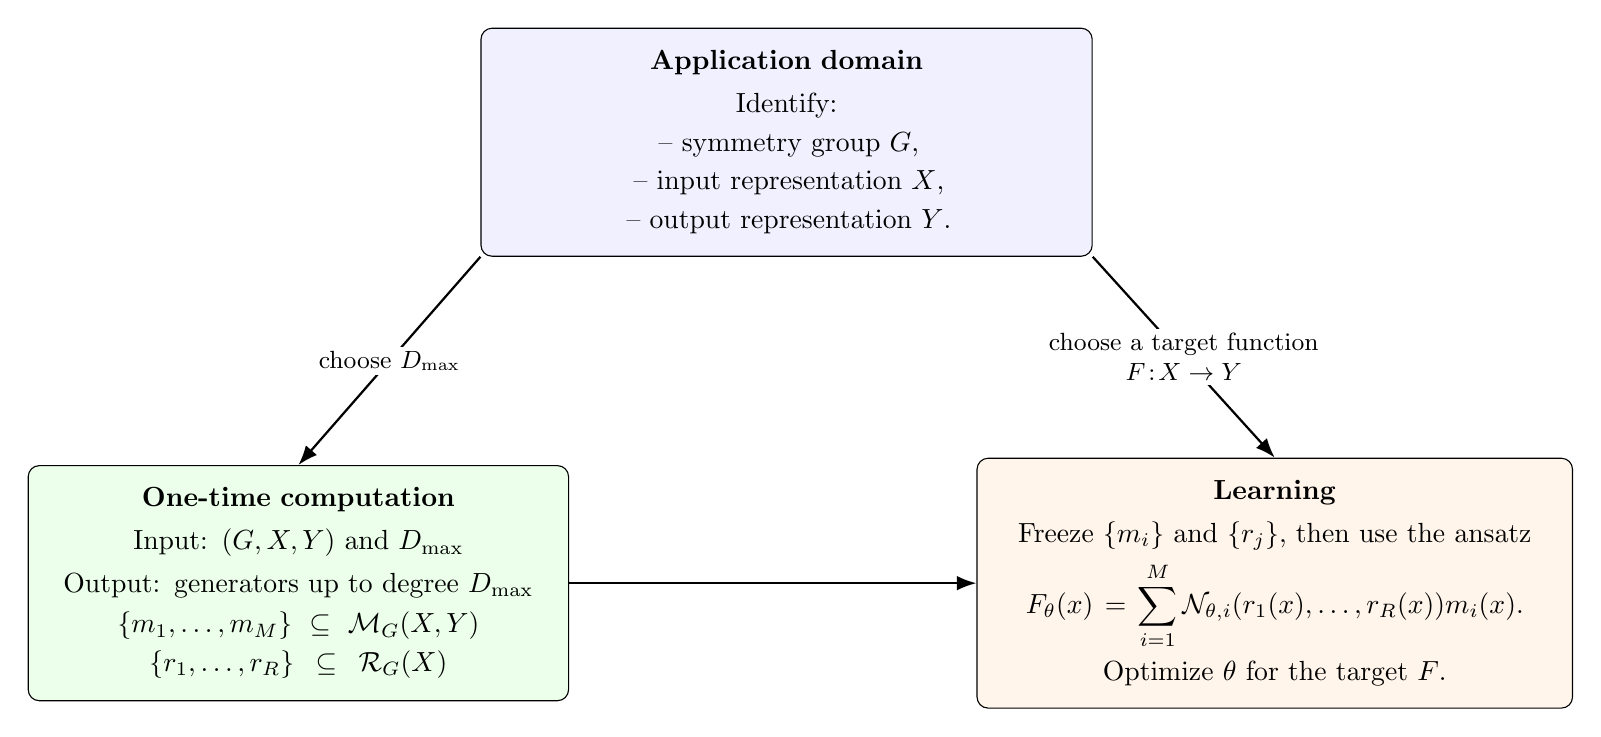
\begin{tikzpicture}[
  every node/.style={font=\normalsize},
  box/.style={draw, rounded corners=4pt, align=center, inner sep=8pt},
  topbox/.style={box, fill=blue!6, text width=7.2cm},
  prebox/.style={box, fill=green!8, text width=6.3cm},
  learnbox/.style={box, fill=orange!8, text width=7.0cm},
  flow/.style={-{Latex[length=2.5mm]}, line width=0.8pt},
  edgelabel/.style={font=\small, fill=white, inner sep=1.5pt, align=center}
]

\node[topbox] (app) at (0,6.2) {\textbf{Application domain}\\[0.35em]
Identify:\\[0.2em]
$\,$-- symmetry group $G$,\\[0.2em]
$\,$-- input representation $X$,\\[0.2em]
$\,$-- output representation $Y$.};

\node[prebox] (pre) at (-6.2,0.6) {\textbf{One-time computation}\\[0.35em]
Input: $(G,X,Y)$ and $D_{\max}$\\[0.35em]
Output: generators up to degree $D_{\max}$\\[0.25em]
$\{m_1,\ldots,m_M\}\subseteq \scM_G(X,Y)$\\[0.2em]
$\{r_1,\ldots,r_R\}\subseteq \scR_G(X)$};

\node[learnbox] (learn) at (6.2,0.6) {\textbf{Learning}\\[0.35em]
Freeze $\{m_i\}$ and $\{r_j\}$, then use the ansatz\\[0.35em]
$\displaystyle F_\theta(x)=\sum_{i=1}^M \scN_{\theta,i}(r_1(x),\dots,r_R(x))m_i(x)$.\\[0.35em]
Optimize $\theta$ for the target $F$.};

\draw[flow] (app.south west) -- node[midway, edgelabel] {choose $D_{\max}$} (pre.north);
\draw[flow] (app.south east) -- node[midway, edgelabel] {\shortstack{choose a target function\\$F\!:\!X\to Y$}} (learn.north);
\draw[flow] (pre.east) -- (learn.west);

\end{tikzpicture}%
}
\caption{Proposed workflow for learning $G$-equivariant functions $F\!:\!X\to Y$.
Starting from an application domain, one identifies the symmetry group $G$, the input representation $X$, and the output representation $Y$.
For the resulting triple $(G,X,Y)$, one chooses a degree bound $D_{\max}$ and performs a one-time computation of covariant generators $\{m_1,\ldots,m_M\}\subseteq \scM_G(X,Y)$ and invariant generators $\{r_1,\ldots,r_R\}\subseteq \scR_G(X)$ up to degree $D_{\max}$.
For any $G$-equivariant target function $F\!:\!X\to Y$, one trains the neural network $\scN_\theta\colon \dsR^R\to\dsR^M$ in Eq.~\eqref{eq:neural-ansatz}.
In particular, for fixed $(G,X,Y)$, the same one-time computation can be reused to learn multiple $G$-equivariant functions from $X$ to $Y$ by training different neural networks.}
\label{fig:equivariant-workflow}
\end{figure}

This paper is organized as follows.
Section~\ref{sec:theory-and-algorithms} describes how we compute minimal generators for the covariant module and invariant algebra.
Section~\ref{sec:examples} works through representative examples in detail.
Section~\ref{sec:conclusion} concludes with suggested directions for future work.
Appendix~\ref{sec:appendix-proofs} provides proofs of our results.

\section{Minimal Integrity Bases for the Covariant Module and Invariant Algebra}\label{sec:theory-and-algorithms}


In this section, we derive an algorithm to compute minimal generators $m_1,\dots,m_M$ for the covariant module and $r_1,\dots,r_R$ for the invariant algebra up to a given degree.
The first step in our approach is to enumerate vector space bases for the homogeneous degree-$D$ pieces
\[
  \scM_G^D(X,Y)\coloneq\left(\scS^D(X^*)\otimes Y\right)^G
\]
and
\[
  \scR_G^D(X)\coloneq\scS^D(X^*)^G
\]
of the covariant module and invariant algebra.
Towards this, suppose that we are given explicit isotypic decompositions
\[
  \begin{aligned}\label{eq:input-output-isotypic}
    X &\cong \bigoplus_{\lambda} H_\lambda\otimes X_\lambda,
    &\quad
    X_\lambda &\coloneq \HomG{H_\lambda}{X},\\
    Y &\cong \bigoplus_{\nu} H_\nu\otimes Y_\nu,
    &\quad
    Y_\nu &\coloneq \HomG{H_\nu}{Y},
  \end{aligned}
\]
for the input and output representations $X$ and $Y$, where $\lambda$ indexes the (isomorphism classes of) irreducible representations of $G$, and $H_\lambda$ is a fixed irreducible representation with label $\lambda$.
The first key observation is that as vector spaces,
\begin{equation}\label{eq:output-reduction}
  \scM_G^D(X,Y)
  \cong
  \bigoplus_{\nu}
  \scM_G^D(X,H_\nu)\otimes Y_\nu,
\end{equation}
so it suffices to study the spaces $\scM_G^D(X,H_\nu)$, i.e., to consider the special case where the output representation $Y = H_\nu$ is irreducible.
The second key observation is that
\begin{equation}\label{eq:duality}
  \scM_G^D(X,H_\nu)
  \cong
  \HomG{H_\nu}{\scS^D(X)}^*,
\end{equation}
which is precisely the dual of the multiplicity space of $H_\nu$ in the isotypic decomposition of $\scS^D(X)$.
Thus, our main technical result, Theorem \ref{thm:isotypic-decomposition}, is an explicit isotypic decomposition of $\scS^D(X)$, which ultimately yields a vector space basis for $\scM_G^D(X,Y)$.

To pass from vector space bases to minimal module or algebra generators, we use a standard procedure based on the graded Nakayama lemma, which applies here since $G$ is linearly reductive, so $\scM_G(X,Y)$ is a finitely generated $\scR_G(X)$-module and $\scR_G(X)$ is a finitely generated $\dsC$-algebra. The basic idea is to proceed degree by degree, using the vector space bases computed above as candidate generators and discarding those that are linearly dependent with products of generators of lower degrees.

In principle, the theory in this work applies whenever $G$ is linearly reductive.
However, in order to implement concrete algorithms, one must provide a model for the irreps of $G$, as well as the following.

\begin{assumption}[Explicit isotypic decompositions of the input and output representations]\label{ass:explicit-isotypic}
  One can provide lists of the active irreducible representations in $X$ and $Y$, bases for the multiplicity spaces $X_\lambda = \HomG{H_\lambda}{X}$ and $Y_\nu = \HomG{H_\nu}{Y}$, and black--box routines for evaluating those basis maps and their adjoints.
\end{assumption}

\begin{assumption}[Explicit Clebsch--Gordan decompositions]\label{ass:explicit-cg}
  One can provide, for each pair of irrep labels $(\lambda_1,\lambda_2)$, a list of the active irreducible representations $H_\gamma$ in $H_{\lambda_1} \otimes H_{\lambda_2}$, a basis for the multiplicity spaces $\HomG{H_\gamma}{H_{\lambda_1} \otimes H_{\lambda_2}}$, and black--box routines for evaluating those basis maps and their adjoints.
\end{assumption}

We adopt these assumptions henceforth.
Our results are summarized in the table below.

\begin{table}[htbp]
  \centering
  \small
  \setlength{\tabcolsep}{5pt}
  \begin{tabular}{>{\raggedright\arraybackslash}p{0.20\textwidth}
    >{\raggedright\arraybackslash}p{0.44\textwidth}
    >{\raggedright\arraybackslash}p{0.29\textwidth}}
    \toprule
    & $Y$ irreducible & $Y$ arbitrary \\
    \midrule
    Vector space basis
    &
    Theorem~\ref{thm:isotypic-decomposition}; Algorithm~\ref{alg:build-isotypic-data-tree}.
    &
    Corollary~\ref{cor:arbitrary-output-basis}; Algorithm~\ref{alg:arbitrary-output-vector-space-basis}.
    \\[0.5em]
    Minimal homogeneous module or algebra generators
    &
    Lemmas~\ref{lem:module-generators} and~\ref{lem:algebra-generators}; Algorithm~\ref{alg:extract-independent-generators}.
    &
    Theorem~\ref{thm:module-generator-reduction}; Algorithm~\ref{alg:arbitrary-output-module-generators}.
    \\
    \bottomrule
  \end{tabular}
  \caption{Overview of results.
  We begin in the top--left corner.
  We use Eq.~\eqref{eq:output-reduction} to move right in the table.
  We use the graded Nakayama lemma to move down in the table.
  To move from the top--left corner to the bottom--right corner, it is algorithmically more efficient to first move down and then move right; i.e., it is more efficient to first use the graded Nakayama lemma to obtain minimal module generators for $\scM_G(X,H_\nu)$ and then use Eq.~\eqref{eq:output-reduction} to lift these generators to $\scM_G(X,Y)$.}
  \label{tab:main-results-guide}
\end{table}


\subsection{Vector Space Bases, Irreducible Outputs}\label{sec:irreducible-bases}

Here, we describe how to obtain a vector space basis for $\scM_G^D(X,H_\nu)$. As motivated above, we begin by bookkeeping an explicit isotypic decomposition of $\scS^D(X)$.

\begin{theorem}[Isotypic decomposition of $\scS^D(X)$]\label{thm:isotypic-decomposition}
  Let
  \[
    X\cong \bigoplus_\lambda H_\lambda\otimes X_\lambda
  \]
  be the isotypic decomposition of $X$, let $\nu\in\dsN_0$, and let $D \in \dsN_0$.
  There is an isomorphism of vector spaces
  \begin{equation}\label{eq:isotypic-decomposition}
    \HomG{H_\nu}{\scS^D(X)} \cong \bigoplus_{(d_\lambda)_\lambda} \bigoplus_{(\pi_\lambda)_\lambda} \bigoplus_{(\mu_\lambda)_\lambda} \HomG{H_\nu}{\bigotimes_\lambda H_{\mu_\lambda}} \otimes \bigotimes_\lambda \HomG{H_{\mu_\lambda}}{e_{\pi_\lambda}(H_\lambda^{\otimes d_\lambda})} \otimes \bigotimes_\lambda e_{\pi_\lambda}^*(X_\lambda^{\otimes d_\lambda}).
  \end{equation}
  where
  \begin{itemize}[leftmargin=2.5em]
    \item $\lambda$ ranges over all (finitely many) nonnegative integers such that $X_\lambda\neq 0$,
    \item $(d_\lambda)_\lambda$ ranges over all sequences of nonnegative integers such that $\sum_\lambda d_\lambda=D$,
    \item $(\pi_\lambda)_\lambda$ ranges over all sequences of integer partitions $\pi_\lambda\vdash d_\lambda$ with at most $\min(\dim H_\lambda,\dim X_\lambda)$ parts,
    \item $(\mu_\lambda)_\lambda$ ranges over all sequences of nonnegative integers such that
    \[
      \HomG{H_\nu}{\bigotimes_\lambda H_{\mu_\lambda}}\neq 0
    \]
    and
    \[
      \HomG{H_{\mu_\lambda}}{e_{\pi_\lambda}(H_\lambda^{\otimes d_\lambda})} \neq 0
    \]
    for all $\lambda$, and
    \item $e_{\pi_\lambda}$ is the Young symmetrizer corresponding to $\pi_\lambda$ (See Definition \ref{def:young-symmetrizer}).
  \end{itemize}
\end{theorem}
\begin{proof}
  See Appendix~\ref{sec:proof-main-decomposition}.
\end{proof}


\begin{definition}[Isotypic data]\label{def:isotypic-data}
  In the context of Theorem \ref{thm:isotypic-decomposition}, a collection of \emph{isotypic data} is a choice of sequences $(d_\lambda)_\lambda$, $(\pi_\lambda)_\lambda$, and $(\mu_\lambda)_\lambda$, along with
  a choice of core tensor
  \[
    C\in \HomG{H_\nu}{\bigotimes_\lambda H_{\mu_\lambda}},
  \]
  leaf tensors
  \[
    L_\lambda\in \HomG{H_{\mu_\lambda}}{H_\lambda^{\otimes d_\lambda}},
  \]
  and tableau tensors
  \[
    T_\lambda\in X_\lambda^{\otimes d_\lambda}.
  \]
  Furthermore, we say that an element $p \in \HomG{H_\nu}{\scS^D(X)}$ corresponds to the above isotypic data if $p$ is the image of
  \[
    C
    \otimes
    \bigotimes_\lambda
    e_{\pi_\lambda} L_\lambda
    \otimes
    \bigotimes_\lambda
    e_{\pi_\lambda}^* T_\lambda
  \]
  under the isomorphism in Eq.~\eqref{eq:isotypic-decomposition}.
\end{definition}

\begin{remark}[Isotypic data tree]\label{rem:isotypic-data-tree}
  A basis for $\HomG{H_\nu}{\scS^D(X)}$ can be obtained by choosing bases for each tensor space in each direct summand on the right-hand-side of Eq.~\eqref{eq:isotypic-decomposition} and transporting the resulting product bases through the isomorphism in Theorem~\ref{thm:isotypic-decomposition}.
  Any such basis is naturally organized by recording the isotypic data of the basis elements in an \emph{isotypic data tree} with levels
  \[
    D \longrightarrow (d_\lambda)_\lambda \longrightarrow (\pi_\lambda)_\lambda \longrightarrow (\mu_\lambda)_\lambda \longrightarrow C, (L_\lambda)_\lambda, (T_\lambda)_\lambda.
  \]
  The interior layers of the isotypic data tree represent the nested direct sum structure in Eq.~\eqref{eq:isotypic-decomposition}, while the final layer stores the core, leaf, and tableau tensors corresponding to the particular basis element via Eq.~\eqref{eq:isotypic-decomposition}.
\end{remark}

\begin{theorem}[Evaluation scheme]\label{thm:evaluation}
  Fix any isotypic data as in Definition \ref{def:isotypic-data}.
  The image of
  \begin{equation}\label{eq:isotypic-data-tensor}
    C
    \otimes
    \bigotimes_\lambda
    e_{\pi_\lambda} L_\lambda
    \otimes
    \bigotimes_\lambda
    e_{\pi_\lambda}^* T_\lambda
  \end{equation}
  under the isomorphism in Eq.~\eqref{eq:isotypic-decomposition} is
  \begin{equation}\label{eq:evaluation}
    p
    =
    \Sym
    \circ
    \left(\bigotimes_\lambda T_\lambda\right)
    \circ
    \left(\bigotimes_\lambda e_{\pi_\lambda} L_\lambda\right)
    \circ
    C,
  \end{equation}
  where the $T_\lambda$ are viewed as maps from $H_\lambda^{\otimes d_\lambda}$ to $X^{\otimes d_\lambda}$.
\end{theorem}
\begin{proof}
  See Appendix~\ref{sec:proof-evaluation}.
\end{proof}

\begin{corollary}\label{cor:evaluation}
  Fix any isotypic data as in Definition \ref{def:isotypic-data}.
  Let the corresponding covariant be
  \[
    p^* \in \scM_G^D(X,H_\nu).
  \]
  Then $p^*$ acts on $x \in X$ by
  \begin{equation}
    p^*(x)
    =
    C^*
    \circ
    \left(\bigotimes_\lambda L_\lambda^*e^*_{\pi_\lambda}\right)
    \circ
    \left(\bigotimes_\lambda T_\lambda^*(x^{\otimes d_\lambda})\right),
  \end{equation}
  where the $T_\lambda^*$ are viewed as maps from $X^{\otimes d_\lambda}$ to $H_\lambda^{\otimes d_\lambda}$.
\end{corollary}
\begin{proof}
  See Appendix~\ref{sec:proof-corollary-evaluation}.
\end{proof}

\begin{remark}\label{rem:isotypic-data-tree-duality}
  In summary, a basis for $\scM_G^D(X,H_\nu)$ is obtained by first constructing an isotypic data tree as in Remark \ref{rem:isotypic-data-tree}, which yields a basis for $\HomG{H_\nu}{\scS^D(X)}$, and then passing that basis through the duality isomorphism in Eq.~\eqref{eq:duality}, which yields a basis for $\scM_G^D(X,H_\nu)$.
  In particular, Corollary \ref{cor:evaluation} describes how to evaluate a polynomial in $\scM_G^D(X,H_\nu)$ given only its isotypic data.
\end{remark}



As noted in Remark \ref{rem:isotypic-data-tree-duality}, the primary step in obtaining a basis for $\scM_G^D(X,H_\nu)$ is to construct an isotypic data tree.
We summarize how to construct this tree in Algorithm \ref{alg:build-isotypic-data-tree} below.

\begin{algorithm}[\texttt{build\_isotypic\_data\_tree}]\label{alg:build-isotypic-data-tree}

  \phantom{}

  \begin{enumerate}[label=\textbf{Step \arabic*.},ref=\arabic*,leftmargin=2.8cm]

    \item[\textbf{Input:}] an isotypic decomposition of $X\cong \bigoplus_\lambda H_\lambda\otimes X_\lambda$, an output irrep label $\nu$, and a degree $D \in \dsN_0$.

    \item[\textbf{Output:}] an isotypic data tree recording a basis for $\scM_G^D(X,H_\nu)$.

    \item \label{alg:build-isotypic-data-tree:step-multidegrees} Enumerate all multidegrees $(d_\lambda)_\lambda$ with $\sum_\lambda d_\lambda=D$.

    \item \label{alg:build-isotypic-data-tree:step-partitions} For each multidegree $(d_\lambda)_\lambda$, enumerate all tuples $(\pi_\lambda)_\lambda$ of partitions $\pi_\lambda\vdash d_\lambda$ with at most $\min(\dim H_\lambda,\dim X_\lambda)$ parts.

    \item \label{alg:build-isotypic-data-tree:step-intermediate-irreps} For each tuple $(\pi_\lambda)_\lambda$, enumerate all tuples of intermediate irreps $(\mu_\lambda)_\lambda$ such that
    \begin{enumerate}[label=\textup{(\alph*)},ref=\theenumi(\alph*),leftmargin=2.2em]
      \item \label{alg:build-isotypic-data-tree:step-schur-constituents} $\HomG{H_{\mu_\lambda}}{e_{\pi_\lambda}(H_\lambda^{\otimes d_\lambda})} \neq 0$ for all $\lambda$ and
      \item \label{alg:build-isotypic-data-tree:step-tensor-product-constituents} $\HomG{H_\nu}{\bigotimes_\lambda H_{\mu_\lambda}}\neq 0$.
    \end{enumerate}

    \item \label{alg:build-isotypic-data-tree:step-bases} For each tuple $(\mu_\lambda)_\lambda$, enumerate
    \begin{enumerate}[label=\textup{(\alph*)},ref=\theenumi(\alph*),leftmargin=2.2em]
      \item \label{alg:build-isotypic-data-tree:step-tensor-train-basis} a tensor-train basis for $\HomG{H_\nu}{\bigotimes_{\lambda} H_{\mu_\lambda}}$;
      \item \label{alg:build-isotypic-data-tree:step-schur-tensor-tree-basis} a tensor-tree basis for each $\HomG{H_{\mu_\lambda}}{e_{\pi_\lambda}(H_\lambda^{\otimes d_\lambda})}$; and
      \item \label{alg:build-isotypic-data-tree:step-ssyt-basis} a semistandard Young tableaux basis for each $e_{\pi_\lambda}^*(X_\lambda^{\otimes d_\lambda})$.
    \end{enumerate}
  \end{enumerate}
\end{algorithm}

We proceed to describe in more detail how we implement each step in Algorithm \ref{alg:build-isotypic-data-tree}.
It is clear how Steps~\ref{alg:build-isotypic-data-tree:step-multidegrees} and~\ref{alg:build-isotypic-data-tree:step-partitions} can be carried out.
Step~\ref{alg:build-isotypic-data-tree:step-schur-constituents} is the plethsym problem, which we resolve computationally by running Algorithm \ref{alg:schur-functor-basis}, \texttt{schur\_functor\_basis}, and retaining the nonempty outputs.
Step~\ref{alg:build-isotypic-data-tree:step-tensor-product-constituents} can be implemented as a consequence of Assumption \ref{ass:explicit-cg}: once the constituent irreps of the binary tensor product of irreps are known, iterating yields the constituent irreps of the n-ary tensor product.
Step~\ref{alg:build-isotypic-data-tree:step-tensor-train-basis} also follows as a consequence of Assumption \ref{ass:explicit-cg}: we make this precise in Algorithm \ref{alg:tensor-product-basis}, \texttt{tensor\_product\_basis}, below.
Step~\ref{alg:build-isotypic-data-tree:step-schur-tensor-tree-basis} is more complicated and is covered by Algorithm \ref{alg:schur-functor-basis}.
Step~\ref{alg:build-isotypic-data-tree:step-ssyt-basis} is a standard result which we record in Lemma \ref{lem:ssyt-basis} below.

\begin{lemma}[Semistandard Young tableaux basis for Schur functors]\label{lem:ssyt-basis}
  Let $V$ be a vector space with basis $(v_1,\dots,v_n)$, and let $\pi\vdash d$ be a partition with at most $n$ parts.
  For each semistandard Young tableau $T$ of shape $\pi$ with entries filled from $\set{1,\dots,n}$, let $v_T\in e_\pi(V^{\otimes d})$ be the image under $e_\pi$ of the simple tensor obtained by reading the entries of $T$ in row major order and replacing each entry $i$ by $v_i$.
  Then the set of all such $v_T$ is a basis for $e_\pi(V^{\otimes d})$.
\end{lemma}
\begin{proof}
  See Weyman~\cite[Proposition~2.1.15(b)]{Weyman2003}.
\end{proof}

We now present the subroutines of Algorithm \ref{alg:build-isotypic-data-tree} in order of increasing complexity.
To begin, by Assumption \ref{ass:explicit-cg}, for any irrep labels $\alpha,\beta,\delta$, we may fix explicit bases $\scB_{\alpha,\beta}^{\delta}$ for $\HomG{H_\delta}{H_\alpha\otimes H_\beta}$.
We call any basis element $c_{\alpha,\beta}^{\delta,a}\in\scB_{\alpha,\beta}^{\delta}$ a \emph{tensor-train core}, where $a$ indexes the basis elements in $\scB_{\alpha,\beta}^{\delta}$.
For any tuple of input irrep labels $\boldsymbol{\lambda}=(\lambda_1,\dots,\lambda_d)$, any tuple of admissible intermediate irrep labels $\boldsymbol{\gamma}=(\gamma_1,\dots,\gamma_d)$ satisfying
\[
  \gamma_1=\lambda_1,
  \qquad
  \HomG{H_{\gamma_{j+1}}}{H_{\gamma_j}\otimes H_{\lambda_{j+1}}}\neq 0
  \qquad
  \text{for } j\in\set{1,\dots,d-1},
\]
and any tuple of basis labels $\boldsymbol{a}=(a_1,\dots,a_{d-1})$, where $a_j$ indexes the basis $\scB_{\gamma_j,\lambda_{j+1}}^{\gamma_{j+1}}$, we define the associated tensor train from $H_{\gamma_d}$ to $H_{\lambda_1}\otimes\cdots\otimes H_{\lambda_d}$ as
\begin{equation}\label{eq:general-tensor-train-map}
  C_{\boldsymbol{\lambda},\boldsymbol{\gamma},\boldsymbol{a}}
  \coloneq
  (c_{\gamma_1,\lambda_2}^{\gamma_2,a_1}\otimes \id)
  \circ
  (c_{\gamma_2,\lambda_3}^{\gamma_3,a_2}\otimes \id)
  \circ\cdots\circ
  c_{\gamma_{d-1},\lambda_d}^{\gamma_d,a_{d-1}}.
\end{equation}
For $d=1$, the unique tensor train is the identity on $H_{\lambda_1}=H_{\gamma_d}$.

\begin{figure}[H]
  \centering
  \resizebox{\textwidth}{!}{%
    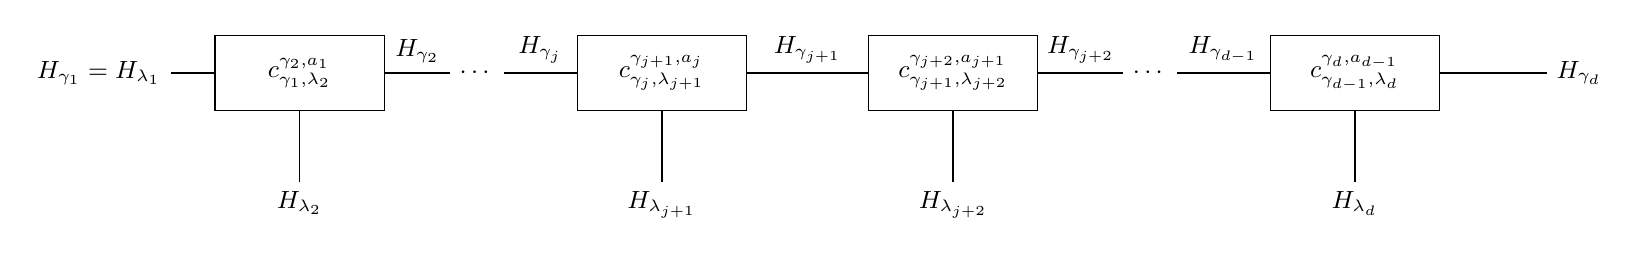
\begin{tikzpicture}[
      core/.style={draw, rectangle, minimum width=2.15cm, minimum height=0.95cm, inner sep=2pt},
      wire/.style={line width=0.55pt},
      every node/.style={font=\small}
    ]
      \node (g1) at (0,0) {$H_{\gamma_1}=H_{\lambda_1}$};
      \node[core] (c1) at (2.55,0) {$c_{\gamma_1,\lambda_2}^{\gamma_2,a_1}$};
      \node (dots1) at (4.8,0) {$\cdots$};
      \node[core] (cj) at (7.15,0) {$c_{\gamma_j,\lambda_{j+1}}^{\gamma_{j+1},a_j}$};
      \node[core] (cjp1) at (10.85,0) {$c_{\gamma_{j+1},\lambda_{j+2}}^{\gamma_{j+2},a_{j+1}}$};
      \node (dots2) at (13.35,0) {$\cdots$};
      \node[core] (cd) at (15.95,0) {$c_{\gamma_{d-1},\lambda_d}^{\gamma_d,a_{d-1}}$};
      \node (gd) at (18.8,0) {$H_{\gamma_d}$};

      \draw[wire] (g1) -- (c1);
      \draw[wire] (c1) -- node[above] {$H_{\gamma_2}$} (dots1);
      \draw[wire] (dots1) -- node[above] {$H_{\gamma_j}$} (cj);
      \draw[wire] (cj) -- node[above] {$H_{\gamma_{j+1}}$} (cjp1);
      \draw[wire] (cjp1) -- node[above] {$H_{\gamma_{j+2}}$} (dots2);
      \draw[wire] (dots2) -- node[above] {$H_{\gamma_{d-1}}$} (cd);
      \draw[wire] (cd) -- (gd);

      \draw[wire] (c1.south) -- ++(0,-0.9) node[below] {$H_{\lambda_2}$};
      \draw[wire] (cj.south) -- ++(0,-0.9) node[below] {$H_{\lambda_{j+1}}$};
      \draw[wire] (cjp1.south) -- ++(0,-0.9) node[below] {$H_{\lambda_{j+2}}$};
      \draw[wire] (cd.south) -- ++(0,-0.9) node[below] {$H_{\lambda_d}$};
    \end{tikzpicture}%
  }
  \caption{Tensor-network diagram for the tensor train in Eq.~\eqref{eq:general-tensor-train-map}.
  Horizontal wires carry the intermediate irreps in the admissible path $\gamma_1\to\cdots\to\gamma_d$.
  Reading the contraction from right to left gives the map $C_{\boldsymbol{\lambda},\boldsymbol{\gamma},\boldsymbol{a}}$.}
  \label{fig:general-tensor-train}
\end{figure}

\begin{proposition}[Tensor-train basis for arbitrary linearly reductive $G$]\label{prop:cg-tensor-train-basis}\label{prop:cg-tensor-train-basis-general}
  Let $G$ be linearly reductive, let $\boldsymbol{\lambda}=(\lambda_1,\dots,\lambda_d)$ be a tuple of irrep labels, and let $\mu$ be an irrep label.
  The maps $C_{\boldsymbol{\lambda},\boldsymbol{\gamma},\boldsymbol{a}}$ in Eq.~\eqref{eq:general-tensor-train-map}, ranging over all admissible intermediate labels $\boldsymbol{\gamma}$ with $\gamma_d=\mu$ and all choices of basis labels $\boldsymbol{a}$, form a basis of
  \[
    \HomG{H_\mu}{H_{\lambda_1}\otimes\cdots\otimes H_{\lambda_d}}.
  \]
\end{proposition}
\begin{proof}
  This is the standard fusion-tree basis.
\end{proof}

\begin{algorithm}[\texttt{tensor\_product\_basis}]\label{alg:tensor-product-basis}
  \phantom{}
  \begin{enumerate}[label=\textbf{Step \arabic*.},leftmargin=2.8cm]
    \item[\textbf{Input:}] an input label tuple $\boldsymbol{\lambda}=(\lambda_1,\dots,\lambda_d)$ and an output label $\mu$.
    \item[\textbf{Output:}] tensor trains representing a basis for $\HomG{H_\mu}{H_{\lambda_1}\otimes\cdots\otimes H_{\lambda_d}}$.
    \item If $d=1$, return the identity tensor train on $H_{\lambda_1}=H_\mu$ if $\lambda_1=\mu$, and return no trains otherwise.
    \item Build the admissible label paths ending at $\mu$.
    Begin with the one-term path $(\lambda_1)$.
    For $j=1,\dots,d-1$, extend each partial path ending in $\gamma_j$ by every irrep label $\gamma_{j+1}$ for which $\scB_{\gamma_j,\lambda_{j+1}}^{\gamma_{j+1}}$ is nonempty.
    After the last extension, discard any path whose final label is not $\mu$.
    \item For each remaining path $\boldsymbol{\gamma}$, choose independently one core $c_{\gamma_j,\lambda_{j+1}}^{\gamma_{j+1},a_j}$ from $\scB_{\gamma_j,\lambda_{j+1}}^{\gamma_{j+1}}$ for each edge $\gamma_j\to\gamma_{j+1}$, and include every possible tuple of such choices.
    \item For each path and choice of cores, form the tensor train $C_{\boldsymbol{\lambda},\boldsymbol{\gamma},\boldsymbol{a}}$ from Eq.~\eqref{eq:general-tensor-train-map}.
    Return the collection of all these tensor trains.
  \end{enumerate}
\end{algorithm}

Next, we describe how to obtain a basis for $\HomG{H_\mu}{e_\pi(H_\lambda^{\otimes d})}$.
We first isolate the cases where $\pi$ is a single row (resp.~a single column).
If $\pi=(d)$ (resp.~$\pi=(1,\dots,1)$), then $e_\pi$ is the row symmetrizer (resp.~column antisymmetrizer), and
\[
  e_\pi(H_\lambda^{\otimes d})
  =
  \begin{cases}
    \Sym^d(H_\lambda), & \pi=(d),\\
    \Lambda^d(H_\lambda), & \pi=(1,\dots,1).
  \end{cases}
\]
In these cases, we first construct a spanning set for $\HomG{H_\mu}{e_\pi(H_\lambda^{\otimes d})}$ using the tensor-train basis for $\HomG{H_\mu}{H_\lambda^{\otimes d}}$ from Algorithm~\ref{alg:tensor-product-basis}.
Then, we evaluate these candidates on random inputs in $H_\lambda^{\otimes d}$ to extract a basis.
We summarize this procedure in Algorithm \ref{alg:symmetrized-power-basis} below.
The probabilistic rank-selection step is the standard polynomial-identity-testing argument: by the Schwartz--Zippel lemma \cite{Schwartz1980,Zippel1979}, a nonzero maximal minor of the formal evaluation matrix is unlikely to vanish on a random finite-field probe batch; see Proposition~\ref{prop:random-rank-test} for the finite-field rank statement used here.

\begin{algorithm}[\texttt{symmetrized\_power\_basis}]\label{alg:symmetrized-power-basis}
  \phantom{}
  \begin{enumerate}[label=\textbf{Step \arabic*.},leftmargin=2.8cm]
    \item[\textbf{Input:}] an irrep label $\lambda$, a degree $d$, an output irrep label $\mu$, and a flag $\varepsilon\in\{\mathrm{sym},\mathrm{antisym}\}$.
    \item[\textbf{Output:}] tensor trains representing a basis for
    \[
      \begin{cases}
        \HomG{H_\mu}{\Sym^d(H_\lambda)}, & \varepsilon=\mathrm{sym},\\
        \HomG{H_\mu}{\Lambda^d(H_\lambda)}, & \varepsilon=\mathrm{antisym}.
      \end{cases}
    \]
    \item If $d=0$, return the scalar train exactly when $H_\mu$ is the trivial representation, and return no trains otherwise.
    \item Enumerate the tensor-train basis for $\HomG{H_\mu}{H_\lambda^{\otimes d}}$ from Algorithm~\ref{alg:tensor-product-basis}.
    \item Choose a probe count $m$ for the rank selection and work over $\dsF_p$ for a prime $p>d$.
    For computations through a maximum degree $D_{\max}$, choose $p>D_{\max}$.
    The current implementation uses primes in the range $1000<p<10000$ as a practical heuristic.
    \item For each probe batch used in the rank selection, do the following.
    \begin{enumerate}[label=\textup{(\alph*)},leftmargin=1.4cm]
      \item If $\varepsilon=\mathrm{sym}$, sample $m$ probes $v^{(a)}\in\dsF_p^{\dim H_\lambda}$ and reuse each probe in all $d$ tensor factors.
      If $\varepsilon=\mathrm{antisym}$, sample $m$ independent $d$-tuples $(v_1^{(a)},\dots,v_d^{(a)})$.
      \item For each candidate tensor train $C$, form the column whose $a$-th output block is
      \[
        \begin{cases}
          C^*(v^{(a)},\dots,v^{(a)}), & \varepsilon=\mathrm{sym},\\
          \displaystyle
          \sum_{\sigma\in\mathfrak S_d}\operatorname{sgn}(\sigma)\,
          C^*(v_{\sigma(1)}^{(a)},\dots,v_{\sigma(d)}^{(a)}),
          & \varepsilon=\mathrm{antisym}.
        \end{cases}
      \]
      \item Flatten the probe and output coordinates, and compute pivot columns over $\dsF_p$.
    \end{enumerate}
    \item Return the tensor trains indexed by the selected pivot columns.
    If no pivot columns are selected, return no trains.
  \end{enumerate}
\end{algorithm}

We are now prepared to handle the case of an arbitrary partition $\pi$.
Let $\pi^\top=(h_1,\dots,h_s)$ be the conjugate partition of $\pi$, so that $h_j$ is the height of the $j$-th column of the row-ordered Young diagram of $\pi$.

\begin{proposition}[Tensor-tree spanning set for Schur powers]\label{prop:general-schur-tree-spanning}
  Let $G$ be linearly reductive, let $\lambda$ and $\mu$ be irrep labels, and let $\pi\vdash d$.
  For each column height $h_j$ and each constituent $\eta_j$ of $\Lambda^{h_j}(H_\lambda)$, choose a basis of
  \[
    \HomG{H_{\eta_j}}{\Lambda^{h_j}(H_\lambda)}.
  \]
  For each tuple $\eta=(\eta_1,\dots,\eta_s)$, choose a tensor-train basis of
  \[
    \HomG{H_\mu}{H_{\eta_1}\otimes\cdots\otimes H_{\eta_s}}
  \]
  from Proposition~\ref{prop:cg-tensor-train-basis}.
  Then the maps
  \[
    H_\mu
    \longrightarrow
    H_{\eta_1}\otimes\cdots\otimes H_{\eta_s}
    \longrightarrow
    \bigotimes_{j=1}^s \Lambda^{h_j}(H_\lambda)
    \xrightarrow{\ r_\pi\ }
    e_\pi(H_\lambda^{\otimes d})
  \]
  span $\HomG{H_\mu}{e_\pi(H_\lambda^{\otimes d})}$ as $\eta$ and the chosen basis elements vary.
\end{proposition}
\begin{proof}
  Since $e_\pi$ is a scalar multiple of $r_\pi c_\pi$, every map $L\in\HomG{H_\mu}{e_\pi(H_\lambda^{\otimes d})}$ can be written as $e_\pi L=r_\pi(c_\pi L)$ up to the nonzero hook-length scalar.
  The image of $c_\pi$ is the column-antisymmetric subspace, canonically identified with $\bigotimes_{j=1}^s\Lambda^{h_j}(H_\lambda)$.
  Decompose each exterior power and then the tensor product of the resulting irreducibles using semisimplicity and Proposition~\ref{prop:cg-tensor-train-basis}.
  This expresses $c_\pi L$, and hence $L$, as a linear combination of the displayed tensor trees.
  Therefore any basis extracted from the displayed spanning set is a basis.
\end{proof}

\begin{algorithm}[\texttt{schur\_functor\_basis}]\label{alg:schur-functor-basis}\label{alg:appendix-leaf-assembly}
  \phantom{}
  \begin{enumerate}[label=\textbf{Step \arabic*.},leftmargin=2.8cm]
    \item[\textbf{Input:}] an irrep label $\lambda$, a partition $\pi\vdash d$, and an output irrep label $\mu$.
    \item[\textbf{Output:}] tensor trees representing a basis for $\HomG{H_\mu}{e_\pi(H_\lambda^{\otimes d})}$.
    \item If $d=0$, return the corresponding scalar tree exactly when $H_\mu$ is the trivial representation, and return no trees otherwise.
    \item If $\pi=(d)$ (resp.~$\pi=(1,\dots,1)$ with $d>1$), call Algorithm~\ref{alg:symmetrized-power-basis} with $\varepsilon=\mathrm{sym}$ (resp.~$\varepsilon=\mathrm{antisym}$), and wrap the selected tensor trains as the corresponding tensor trees.
    \item In the general case, let $\pi^\top=(h_1,\dots,h_s)$.
    Enumerate tuples $(\eta_1,\dots,\eta_s)$ such that Algorithm~\ref{alg:symmetrized-power-basis} returns a nonempty basis for each $\HomG{H_{\eta_j}}{\Lambda^{h_j}(H_\lambda)}$ and Algorithm~\ref{alg:tensor-product-basis} returns a nonempty basis for $\HomG{H_\mu}{H_{\eta_1}\otimes\cdots\otimes H_{\eta_s}}$.
    \item For every such tuple, combine an interior tensor train for $\HomG{H_\mu}{H_{\eta_1}\otimes\cdots\otimes H_{\eta_s}}$ with the leaf tensor trains returned for the exterior-power spaces $\HomG{H_{\eta_j}}{\Lambda^{h_j}(H_\lambda)}$.
    \item Apply the row symmetrizer and rank-select a basis from the resulting tensor trees using the evaluation routine.
    Return the selected trees.
  \end{enumerate}
\end{algorithm}



Finally, it remains to describe how to evaluate the polynomials given their isotypic data.
The only subtle point is the row symmetrizer in the semistandard Young tableau factor.
A row with distinct labels $\kappa_1,\dots,\kappa_r$ and multiplicities $d_1,\dots,d_r$ is governed by the monomial
\[
  x_1^{d_1}\cdots x_r^{d_r}.
\]
Its Waring decomposition gives a symmetric CP decomposition of the corresponding row-symmetrized tensor, replacing an expansion over the row stabilizer by a sum over the Waring grid.

\begin{lemma}[Monomial Waring grid]\label{lem:waring-monomial-matrix}
  Let
  \[
    F=x_1^{d_1}\cdots x_r^{d_r},
    \qquad
    d=d_1+\cdots+d_r.
  \]
  For $j_i\in\{0,\dots,d_i\}$, let $W$ have rows
  \[
    j=(j_1,\dots,j_r)
  \]
  and let
  \[
    b_j=\prod_{i=1}^r (-1)^{d_i-j_i}\binom{d_i}{j_i}.
  \]
  Then
  \begin{equation}\label{eq:waring-monomial}
    \sum_{\textup{rows }j\textup{ of }W}
      b_j(j_1x_1+\cdots+j_rx_r)^d
    =
    d!F,
  \end{equation}
  so $W$ has $\prod_i(d_i+1)$ rows.
  In finite-field mode this identity is used with characteristic $p>d$ so that the degree factorial is nonzero.
  The implementation uses the unnormalized left-hand side of \eqref{eq:waring-monomial}; as with the other randomized finite-field rank tests, very small primes may still give bad reductions.
\end{lemma}
\begin{proof}
  This is the mixed finite-difference identity applied to the homogeneous polynomial $(t_1x_1+\cdots+t_rx_r)^d$.
\end{proof}

\begin{proposition}[Waring grid evaluation of a row symmetrizer]\label{prop:waring-grid-evaluation}
  Let $V$ and $Y$ be complex vector spaces, let $M:V^{\otimes d}\to Y$ be linear, and let
  \[
    P_d=\frac{1}{d!}\sum_{\sigma\in\mathfrak S_d}\sigma
  \]
  be the symmetrizer on $V^{\otimes d}$.
  For vectors $v_1,\dots,v_r\in V$, let $W$ and $b$ be the Waring grid and coefficient vector from Lemma~\ref{lem:waring-monomial-matrix} for the exponents $d_1,\dots,d_r$.
  For each row $j=(j_1,\dots,j_r)$ of $W$, write $b_j$ for the matching entry of $b$ and set
  \[
    u_j=\sum_{i=1}^r j_i v_i.
  \]
  Then
  \begin{equation}\label{eq:waring-row-evaluation}
    M\!\left(P_d(v_1^{\otimes d_1}\otimes\cdots\otimes v_r^{\otimes d_r})\right)
    =
    \frac{1}{d!}
    \sum_{\textup{rows }j\textup{ of }W} b_j\,M(u_j^{\otimes d}).
  \end{equation}
\end{proposition}
\begin{proof}
  Lemma~\ref{lem:waring-monomial-matrix} is an identity in $\Sym^d(\dsC^r)$.
  Apply the linear map $\dsC^r\to V$ sending the $i$-th standard basis vector to $v_i$, then use the standard symmetrization embedding $\Sym^d(V)\hookrightarrow V^{\otimes d}$.
  Applying the linear map $M$ gives Eq.~\eqref{eq:waring-row-evaluation}.
  The Waring identity used in the first step is exactly the one cited from Buczy\'nska--Buczy\'nski--Teitler in Lemma~\ref{lem:waring-monomial-matrix}.
\end{proof}

Applying Proposition~\ref{prop:waring-grid-evaluation} independently to the rows of a tableau replaces the row part of the Young symmetrizer, whose direct expansion has $|R_\pi|$ terms, by the Cartesian product of the row Waring grids.
Consequently, the number of tensor-train evaluations is controlled by the number of rank-one terms in the symmetric CP decompositions of the row monomials.

The evaluation procedure below is Corollary~\ref{cor:evaluation} written with the Waring-grid identity.
Including the normalizing factor in Eq.~\eqref{eq:waring-monomial} gives the normalized value of the chosen Young symmetrizer.

\begin{algorithm}[Evaluation from isotypic data]\label{alg:evaluate-basis}

  \phantom{}

  \begin{enumerate}[label=\textbf{Step \arabic*.},leftmargin=2.8cm]

    \item[\textbf{Input:}] isotypic data for a polynomial $p^* \in \scM_G^D(X,H_\nu)$ and a point $x \in X$.

    \item[\textbf{Output:}] the evaluation $p^*(x) \in H_\nu$.

    \item Decompose $x$ according to the isotypic decomposition of $X$.
    Equivalently, for each active input irrep $\lambda$, form the multiplicity-indexed tuple
    \[
      x_\lambda=(x_{\lambda,1},\dots,x_{\lambda,\dim X_\lambda}),
      \qquad
      x_{\lambda,i}\in H_\lambda.
    \]

    \item For each $\lambda$,
    \begin{enumerate}[label=\textup{(\alph*)},leftmargin=2.2em]
      \item Let the chosen tableau tensor $T_\lambda$ be represented by an SSYT $\tau_\lambda$.
      For each row of $\tau_\lambda$, read off the distinct multiplicity labels $\kappa=(\kappa_1,\dots,\kappa_r)$ and their powers $\alpha=(\alpha_1,\dots,\alpha_r)$.

      \item Form the Waring grid $W$ and coefficient vector $b$ for $\alpha$ using Lemma~\ref{lem:waring-monomial-matrix}.
      Compute the row-linear combinations
      \[
        U_{\mathrm{row}}(w)
        =
        \sum_{i=1}^r w_i\,x_{\lambda,\kappa_i}
        \in H_\lambda
      \]
      for the rows $w=(w_1,\dots,w_r)$ of $W$, with coefficient $b_w$.

      \item Evaluate each column leaf tensor train in the tensor-tree representation of $L_\lambda^*$ on the relevant row-linear combinations, using the explicit alternating sum for the column antisymmetrizer.
      If a column has height $h$, this uses the Waring-grid rows attached to the first $h$ tableau rows.

      \item Evaluate the interior tensor train of $L_\lambda^*$ on the column-leaf outputs.
      The same Waring-grid row is shared across every tensor slot belonging to a tableau row.
      Sum over all choices of Waring-grid rows, weighted by the product of the corresponding coefficients $b_w$, and include the normalizing constants from Eq.~\eqref{eq:waring-monomial} if normalized Young symmetrizers are desired.
      The result is
      \[
        h_{\mu_\lambda}
        =
        L_\lambda^*e_{\pi_\lambda}^*T_\lambda^*(x_\lambda^{\otimes d_\lambda})
        \in H_{\mu_\lambda}.
      \]
    \end{enumerate}

    \item Evaluate the core tensor train:
    \[
      p^*(x)
      =
      C^*\left(\bigotimes_\lambda h_{\mu_\lambda}\right)
      \in H_\nu.
    \]
  \end{enumerate}
\end{algorithm}



\subsection{Vector Space Bases, Arbitrary Outputs}\label{sec:arbitrary-bases}

In this section, we describe how to obtain a vector space basis for $\scM_G^D(X,Y)$ using Eq.~\eqref{eq:output-reduction}.
Concretely, the isomorphism in Eq.~\eqref{eq:output-reduction} is just composition: given a polynomial $p^* \in \scM_G^D(X,H_\nu)$ and a map $q \in Y_\nu = \HomG{H_\nu}{Y}$, the corresponding polynomial in $\scM_G^D(X,Y)$ is the composition $q \circ p^*$.
Thus, we have the following corollary.

\begin{corollary}[Basis for $\scM_G^D(X,Y)$]\label{cor:arbitrary-output-basis}
  Let
  \[
    Y\cong \bigoplus_{\nu} H_\nu\otimes Y_\nu
  \]
  be the isotypic decomposition of $Y$, let $B_\nu$ be bases for the $\scM_G^D(X,H_\nu)$, let $C_\nu$ be bases for the $Y_\nu$, and let $D\in\dsN_0$.
  Then the simple tensors
  \[
    \bigcup_{\nu}\{p^*\otimes q : p^*\in B_\nu,\ q\in C_\nu\}
  \]
  form a basis for $\scM_G^D(X,Y)$ under the isomorphism in Eq.~\eqref{eq:output-reduction}.
\end{corollary}


\begin{algorithm}[Arbitrary-output vector-space basis]\label{alg:arbitrary-output-vector-space-basis}

  \phantom{}

  \begin{enumerate}[label=\textbf{Step \arabic*.},leftmargin=2.8cm]

    \item[\textbf{Input:}] isotypic decompositions
    \[
      X\cong \bigoplus_\lambda H_\lambda\otimes X_\lambda,
      \quad
      Y\cong \bigoplus_\nu H_\nu\otimes Y_\nu,
    \]
    and a degree $D \in \dsN_0$.

    \item[\textbf{Output:}] a vector space basis for $\scM_G^D(X,Y)$.

    \item For each $\nu$ such that $Y_\nu\neq 0$,

    \begin{enumerate}
      \item run Algorithm~\ref{alg:build-isotypic-data-tree} on $(X,\nu,D)$ to enumerate a basis $B_\nu$ for $\scM_G^D(X,H_\nu)$;

      \item enumerate a basis $C_\nu$ for the multiplicity space $Y_\nu$.
    \end{enumerate}

    \item Return the $B_\nu$ and the $C_\nu$.
  \end{enumerate}
\end{algorithm}



\subsection{Minimal Integrity Bases, Irreducible Outputs}\label{sec:irreducible-generators}

In this section, we use the graded Nakayama lemma to obtain minimal homogeneous module and algebra generators for $\scM_G(X,H_\nu)$ and $\scR_G(X)$ up to a given degree.

\begin{assumption}\label{ass:finitely-generated}
  The covariant module $\scM_G(X,Y)$ is a finitely generated $\scR_G(X)$-module, and the invariant algebra $\scR_G(X)$ is a finitely generated $\dsC$-algebra.
\end{assumption}


\begin{lemma}[Graded Nakayama lemma, module generators]\label{lem:module-generators}
  Let $L\subseteq \scM_G(X,Y)$ be a homogeneous subset.
  The following are equivalent:
  \begin{enumerate}[label=\textup{(\roman*)}, leftmargin=2em]
    \item $L$ is a minimal homogeneous generating set of $\scM_G(X,Y)$ as an $\scR_G(X)$-module.
    \item The image of $L$ is a basis for $\scM_G(X,Y)\big/\scR_{G,+}(X)\scM_G(X,Y)$.
    \item For every $D\in\dsN_0$, the degree-$D$ elements in $L$ form a basis for a complement of
    \[
      \left(\scR_{G,+}(X)\scM_G(X,Y)\right)^D
    \]
    inside $\scM_G^D(X,Y)$.
  \end{enumerate}
  Moreover, if $R^D$ and $M^D$ are vector space bases for $\scR_G^{D}(X)$ and $\scM_G^D(X,Y)$, then
  \[
    \begin{aligned}
      \left(\scR_{G,+}(X)\scM_G(X,Y)\right)^D
      &=
      \sum_{D'=1}^{D-1} \scR_G^{D'}(X)\,\scM_G^{D-D'}(X,Y) \\
      &=
      \Span\left\{r m \mid r \in R^{D'},\ m \in M^{D-D'},\ D' \in \set{1,\dots,D-1}\right\} \\
      &=
      \Span\left\{r l \mid r \in R^{D'},\ l \in L^{D-D'},\ D' \in \set{1,\dots,D-1}\right\}.
    \end{aligned}
  \]
\end{lemma}
\begin{proof}
  \textup{(i)} $\iff$ \textup{(ii)}: This is the graded Nakayama lemma \cite[Lemma 10.56.1]{Stacks0EKB}.
  \textup{(ii)} $\iff$ \textup{(iii)}: This holds since $L$ is homogeneous.
\end{proof}

\begin{lemma}[Graded Nakayama lemma, algebra generators]\label{lem:algebra-generators}
  Let $L\subseteq \scR_{G,+}(X)$ be a homogeneous subset.
  The following are equivalent:
  \begin{enumerate}[label=\textup{(\roman*)}, leftmargin=2em]
    \item $L$ is a minimal homogeneous generating set of $\scR_G(X)$ as a $\dsC$-algebra.
    \item The image of $L$ is a basis for $\scR_{G,+}(X)\big/\scR_{G,+}(X)^2$.
    \item For every $D\in\dsN$, the degree-$D$ elements in $L$ form a basis for a complement of $\left(\scR_{G,+}(X)^2\right)^D$ inside $\scR_G^D(X)$.
  \end{enumerate}
  Moreover, if $R^D$ are vector space bases for $\scR_G^D(X)$, then
  \[
    \begin{aligned}
      \left(\scR_{G,+}(X)^2\right)^D
      &=
      \sum_{D'=1}^{\lfloor D/2\rfloor} \scR_G^{D'}(X)\,\scR_G^{D-D'}(X) \\
      &=
      \Span\left\{s r \mid s\in R^{D'},\ r\in R^{D-D'},\ D'\in \set{1,\dots,\lfloor D/2\rfloor}\right\} \\
      &=
      \Span\left\{l r \mid l\in L^{D'},\ r\in R^{D-D'},\ D'\in \set{1,\dots,\lfloor D/2\rfloor}\right\}.
    \end{aligned}
  \]
\end{lemma}
\begin{proof}
  Apply \cite[Lemma 10.56.1]{Stacks0EKB} to the graded $\scR_G(X)$-module $\scR_{G,+}(X)$.
  It remains to show that for homogeneous subsets $L\subseteq \scR_{G,+}(X)$, generating $\scR_G(X)$ as a $\dsC$-algebra is equivalent to generating $\scR_{G,+}(X)$ as an $\scR_G(X)$-module.

  First suppose that $L$ generates $\scR_G(X)$ as a $\dsC$-algebra.
  Then every element of $\scR_{G,+}(X)$ is a $\dsC$-linear combination of monomials in elements of $L$.
  Every such monomial has positive total degree, so it contains at least one factor from $L$; factoring out one such term shows that the monomial lies in $L \cdot \scR_G(X)$.
  Hence $L$ generates $\scR_{G,+}(X)$ as an $\scR_G(X)$-module.

  Conversely, suppose that $L$ generates $\scR_{G,+}(X)$ as an $\scR_G(X)$-module, and let $A\subseteq \scR_G(X)$ be the $\dsC$-subalgebra generated by $L$.
  We show by induction on $D$ that
  \[
    \bigoplus_{d=0}^{D} \scR_G^d(X)\subseteq A.
  \]
  This is clear for $D=0$.
  Assume it holds through degree $D-1$, and let $f\in \scR_G^D(X)\subseteq \scR_{G,+}(X)$.
  Since $L$ generates $\scR_{G,+}(X)$ as an $\scR_G(X)$-module, we can write
  \[
    f=\sum_i r_i\ell_i,
    \qquad
    \ell_i\in L,
  \]
  with each $r_i$ homogeneous of degree $D-\deg \ell_i < D$.
  By the induction hypothesis, every $r_i$ lies in $A$, and each $\ell_i$ lies in $A$ by construction, so $f\in A$.
  Thus $\scR_G^D(X)\subseteq A$, completing the induction.
  Therefore $A=\scR_G(X)$, so $L$ generates $\scR_G(X)$ as a $\dsC$-algebra.
\end{proof}


The implementation uses one generator-extraction routine.
The caller chooses the target graded space, the probe-count rule, and the range of previous generator degrees, analogous to the Schur-power special cases where the same rank-selection routine is called with the symmetric or antisymmetric flag.

\begin{algorithm}[\texttt{extract\_independent\_generators}]\label{alg:extract-independent-generators}

  \phantom{}
  \begin{enumerate}[label=\textbf{Step \arabic*.},leftmargin=2.8cm]

    \item[\textbf{Input:}] a flag $\kappa\in\{\mathrm{module},\mathrm{algebra}\}$; vector space bases for $\scR_G^D(X)$ for all $D=0,\dots,D_{\max}$; and vector space bases for a target graded space $\scT^D$ for all $D=0,\dots,D_{\max}$, where
    \[
      \scT^D=
      \begin{cases}
        \scM_G^D(X,H_\nu), & \kappa=\mathrm{module},\\
        \scR_G^D(X), & \kappa=\mathrm{algebra}.
      \end{cases}
    \]

    \item[\textbf{Output:}] selected homogeneous target generators up to degree $D_{\max}$: minimal module generators for $\scM_G(X,H_\nu)$ over $\scR_G(X)$ when $\kappa=\mathrm{module}$, and, when $\kappa=\mathrm{algebra}$, the positive-degree minimal algebra generators for $\scR_G(X)$ over $\dsC$ together with the initialized degree-$0$ block.

    \item Set
    \[
      q=
      \begin{cases}
        \dim H_\nu, & \kappa=\mathrm{module},\\
        1, & \kappa=\mathrm{algebra},
      \end{cases}
      \qquad
      m_D=
      \begin{cases}
        \left\lceil \dim\scT^D/q\right\rceil, & \kappa=\mathrm{module},\\
        \dim\scT^D, & \kappa=\mathrm{algebra}.
      \end{cases}
    \]
    Also set
    \[
      J_D=
      \begin{cases}
        \{0,\dots,D-1\}, & \kappa=\mathrm{module},\\
        \{1,\dots,\lfloor D/2\rfloor\}, & \kappa=\mathrm{algebra}.
      \end{cases}
    \]

    \item Select a batch of random probes $x^{(1)},\dots,x^{(m)}\in X$ with
    \[
      m\ge \max_{D=0,\dots,D_{\max}} m_D,
    \]
    in accordance with Proposition~\ref{prop:random-rank-test}.

    \item Evaluate the invariant basis elements on these probes to form syndrome matrices for $\scR_G^D(X)$, and initialize the selected degree-$0$ target generators to be the whole basis of $\scT^0$.

    \item For each degree $D=1,\dots,D_{\max}$, use only the first $m_D$ probes and form the previous-generator product blocks
    \[
      \scR_G^{D-g}(X)\,\scG^g,
      \quad g\in J_D,
    \]
    where $\scG^g\subseteq\scT^g$ denotes the target generators already selected in degree $g$.
    Each block is represented by the row-wise Kronecker product of the degree-$D-g$ invariant syndrome matrix and the degree-$g$ selected-generator syndrome matrix.
    Empty blocks are omitted.

    \item Evaluate the full target basis $\scT^D$ on the same $m_D$ probes.
    Concatenate the previous-generator product blocks first and this degree-$D$ target block last.

    \item Compute the pivot columns of the concatenated syndrome matrix.

    \item Retain only those pivots lying in the final target block.
    Record the corresponding basis elements as $\scG^D\subseteq\scT^D$, cache their syndrome matrices for later degrees, and collect the selected generators over all degrees $D=0,\dots,D_{\max}$.
  \end{enumerate}
\end{algorithm}



\subsection{Minimal Integrity Bases, Arbitrary Outputs}\label{sec:arbitrary-generators}

In this section, we use Eq.~\eqref{eq:output-reduction} to generalize the results in the previous section and obtain minimal homogeneous module generators for covariant modules $\scM_G(X,Y)$ with arbitrary output space $Y$.


\begin{theorem}[]\label{thm:module-generator-reduction}
  Let
  \[
    Y\cong \bigoplus_{\nu} H_\nu\otimes Y_\nu
  \]
  be the isotypic decomposition of $Y$, let $L_\nu \subseteq \scM_G(X,H_\nu)$ be homogeneous subsets, and let $C_\nu$ be bases for the $Y_\nu$.
  Then Eq.~\eqref{eq:output-reduction} induces a canonical isomorphism of graded $\scR_G(X)$-modules
  \begin{equation}\label{eq:module-generator-reduction-iso}
    \scM_G(X,Y)\cong\bigoplus_{\nu}\scM_G(X,H_\nu)\otimes Y_\nu.
  \end{equation}
  Moreover, the following are equivalent:
  \begin{enumerate}[label=\textup{(\roman*)}]
    \item every $L_\nu$ is a minimal homogeneous generating set of $\scM_G(X,H_\nu)$ as an $\scR_G(X)$-module;
    \item the preimage in $\scM_G(X,Y)$ of
    \[
      \widetilde L\coloneq \bigcup_{\nu:\,Y_\nu\neq 0}\{m\otimes b : m\in L_\nu,\ b\in C_\nu\}
    \]
    under the isomorphism \eqref{eq:module-generator-reduction-iso} is a minimal homogeneous generating set of $\scM_G(X,Y)$ as an $\scR_G(X)$-module.
  \end{enumerate}
\end{theorem}

\begin{proof}
  Summing Eq.~\eqref{eq:output-reduction} over all degrees $D\ge 0$ gives a canonical isomorphism of graded vector spaces
  \[
    \scM_G(X,Y)
    =
    \bigoplus_{D\ge 0}\scM_G^D(X,Y)
    \cong
    \bigoplus_{D\ge 0}\bigoplus_{\nu}\scM_G^D(X,H_\nu)\otimes Y_\nu
    \cong
    \bigoplus_{\nu}\scM_G(X,H_\nu)\otimes Y_\nu.
  \]
  This isomorphism is $\scR_G(X)$-linear, because multiplication by an invariant polynomial acts only on the $\scM_G(X,H_\nu)$-factor.
  This proves \eqref{eq:module-generator-reduction-iso}.

  For each $\nu$, set
  \[
    Q_\nu\coloneq \scM_G(X,H_\nu)\big/\scR_{G,+}(X)\scM_G(X,H_\nu).
  \]
  Since $Y_\nu$ is a multiplicity space, it carries the trivial $G$-action and is concentrated in degree $0$.
  Hence $\scR_{G,+}(X)$ acts only on the first tensor factor, so
  \[
    \scR_{G,+}(X)\bigl(\scM_G(X,H_\nu)\otimes Y_\nu\bigr)
    =
    \scR_{G,+}(X)\scM_G(X,H_\nu)\otimes Y_\nu.
  \]
  Therefore,
  \[
    \bigl(\scM_G(X,H_\nu)\otimes Y_\nu\bigr)\Big/\scR_{G,+}(X)\bigl(\scM_G(X,H_\nu)\otimes Y_\nu\bigr)
    \cong
    Q_\nu\otimes Y_\nu.
  \]
  Applying this for all $\nu$ and using \eqref{eq:module-generator-reduction-iso}, we obtain an isomorphism
  \[
    \scM_G(X,Y)\big/\scR_{G,+}(X)\scM_G(X,Y)
    \cong
    \bigoplus_{\nu} Q_\nu\otimes Y_\nu.
  \]

  Assume \textup{(i)}.
  By Lemma~\ref{lem:module-generators}, the image $\overline{L_\nu}$ of $L_\nu$ in $Q_\nu$ is a basis for every $\nu$ with $Y_\nu\neq 0$.
  Since $C_\nu$ is a basis of $Y_\nu$, the simple tensors
  \[
    \{\overline{m}\otimes b : m\in L_\nu,\ b\in C_\nu\}
  \]
  form a basis of $Q_\nu\otimes Y_\nu$.
  Taking the union over $\nu$ yields a basis of
  \[
    \bigoplus_{\nu} Q_\nu\otimes Y_\nu
    \cong
    \scM_G(X,Y)\big/\scR_{G,+}(X)\scM_G(X,Y).
  \]
  Hence the image in $\scM_G(X,Y)/\scR_{G,+}(X)\scM_G(X,Y)$ of the preimage of $\widetilde L$ under \eqref{eq:module-generator-reduction-iso} is a basis.
  Another application of Lemma~\ref{lem:module-generators} shows that this preimage is a minimal homogeneous generating set of $\scM_G(X,Y)$ over $\scR_G(X)$.
  Thus \textup{(ii)} holds.

  Conversely, assume \textup{(ii)}.
  By Lemma~\ref{lem:module-generators}, the image of $\widetilde L$ is a basis of
  \[
    \bigoplus_{\nu} Q_\nu\otimes Y_\nu.
  \]
  For each fixed $\nu$, the choice of basis $C_\nu$ gives a direct-sum decomposition
  \[
    Q_\nu\otimes Y_\nu
    =
    \bigoplus_{b\in C_\nu} Q_\nu\otimes \dsC b.
  \]
  Hence
  \[
    \bigoplus_{\nu} Q_\nu\otimes Y_\nu
    =
    \bigoplus_{\nu}\bigoplus_{b\in C_\nu} Q_\nu\otimes \dsC b.
  \]
  The basis $\widetilde L$ is the disjoint union of the subsets
  \[
    \{\overline{m}\otimes b : m\in L_\nu\}
    \subseteq
    Q_\nu\otimes \dsC b.
  \]
  Since these subsets lie in distinct direct summands and their union is a basis of the whole direct sum, each subset
  \[
    \{\overline{m}\otimes b : m\in L_\nu\}
  \]
  is a basis of $Q_\nu\otimes \dsC b$.
  For any fixed nonzero $b\in C_\nu$, the map
  \[
    Q_\nu \longrightarrow Q_\nu\otimes \dsC b,
    \quad
    q\longmapsto q\otimes b,
  \]
  is an isomorphism of vector spaces.
  Therefore $\overline{L_\nu}$ is a basis of $Q_\nu$.
  By Lemma~\ref{lem:module-generators}, each $L_\nu$ is a minimal homogeneous generating set of $\scM_G(X,H_\nu)$ over $\scR_G(X)$.
  Thus \textup{(i)} holds.
\end{proof}



\begin{algorithm}[Arbitrary-output module generators]\label{alg:arbitrary-output-module-generators}

  \phantom{}
  \begin{enumerate}[label=\textbf{Step \arabic*.},leftmargin=2.8cm]

    \item[\textbf{Input:}] isotypic decompositions
    \[
      X\cong \bigoplus_\lambda H_\lambda\otimes X_\lambda,
      \quad
      Y\cong \bigoplus_\nu H_\nu\otimes Y_\nu,
    \]
    and a degree bound $D_{\max}\in\dsN_0$.

    \item[\textbf{Output:}] minimal homogeneous module generators for $\scM_G(X,Y)$ over $\scR_G(X)$ up to degree $D_{\max}$.

    \item Compute vector space bases for $\scR_G^D(X)$ for all $D=0,\dots,D_{\max}$.

    \item For each $\nu$ such that $Y_\nu\neq 0$,
    \begin{enumerate}[leftmargin=2.2em]
      \item compute vector space bases for $\scM_G^D(X,H_\nu)$ for all $D=0,\dots,D_{\max}$ using Section~\ref{sec:irreducible-bases};
      \item run Algorithm~\ref{alg:extract-independent-generators} in the module setting with $Y=H_\nu$ to obtain a minimal homogeneous generating set $L_\nu\subseteq \scM_G(X,H_\nu)$ up to degree $D_{\max}$; and
      \item choose a basis $C_\nu$ of the multiplicity space $Y_\nu$.
    \end{enumerate}

    \item Return
    \[
      \widetilde L\coloneq \bigcup_{\nu:\,Y_\nu\neq 0}\{m\otimes b : m\in L_\nu,\ b\in C_\nu\}.
    \]
  \end{enumerate}
\end{algorithm}



\section{Examples}\label{sec:examples}

\subsection{\texorpdfstring{$\SO(2)$}{SO(2)}}\label{sec:examples-so2}

Let $G=\SO(2)=\{e^{i\theta}:\theta\in\dsR\}$, so the irreps $H_\lambda$, $\lambda\in\dsZ$, are one-dimensional and correspond to the characters
\begin{equation*}
  \chi_\lambda(e^{i\theta})=e^{i\lambda\theta}.
\end{equation*}
The Clebsch--Gordan decomposition is
\begin{equation}\label{eq:so2-Clebsch--Gordan}
  H_\lambda\otimes H_\mu\cong H_{\lambda+\mu}.
\end{equation}
Moreover, let $\pi\vdash d$.
Since $H_\lambda$ is one-dimensional,
\begin{equation}\label{eq:so2-schur-power}
  e_\pi(H_\lambda^{\otimes d})
  =
  \begin{cases}
    H_{d\lambda}, & \pi=(d),\\
    0, & \text{otherwise}.
  \end{cases}
\end{equation}
Specializing Theorem~\ref{thm:isotypic-decomposition} to this setting gives the following Corollary.

\begin{corollary}[Theorem~\ref{thm:isotypic-decomposition} for $\SO(2)$]\label{cor:so2-isotypic-decomposition}
  Let
  \[
    X\cong \bigoplus_{\lambda}H_\lambda\otimes X_\lambda
  \]
  be the $\SO(2)$-isotypic decomposition of a finite-dimensional representation.
  Then for every $\nu\in\dsZ$ and $D\in\dsN_0$,
  \[
    \operatorname{Hom}_{G}(H_\nu,\scS^D(X))
    \cong
    \bigoplus_{(d_\lambda)_{\lambda}}
    \bigotimes_{\lambda}\Sym^{d_\lambda}(X_\lambda),
  \]
  where $(d_\lambda)_\lambda$ ranges over all sequences of nonnegative integers such that $\sum_\lambda d_\lambda=D$ and $\sum_\lambda \lambda d_\lambda=\nu$.
  Consequently, a basis for $\scM_G^D(X,H_\nu)$ is indexed by monomials in the multiplicity variables whose total $G$-weight is $\nu$.
\end{corollary}
\begin{proof}
  Substitute Equations~\eqref{eq:so2-Clebsch--Gordan} and~\eqref{eq:so2-schur-power} into Theorem~\ref{thm:isotypic-decomposition} and apply Schur's lemma to conclude that the nonzero summands must have
  \[
    \pi_\lambda=(d_\lambda),\qquad
    \mu_\lambda=\lambda d_\lambda,\qquad
    \sum_\lambda \lambda d_\lambda=\nu,
  \]
  which gives the displayed decomposition.
\end{proof}

\begin{remark}
  Taking $\nu=0$ in Corollary~\ref{cor:so2-isotypic-decomposition} gives the usual monomial basis for the invariant ring: after choosing coordinates in each multiplicity space, the invariant monomials are precisely those whose exponent vector has total weight zero \cite[\S 1.4, Lemma~1.4.2]{Sturmfels2008}.
\end{remark}

\subsection{\texorpdfstring{$\Orth(2)$}{O(2)}}\label{sec:examples-o2}

Let $G=\Orth(2)$.
Its irreducible representations are labeled by
\[
  +,\quad -,\quad 1,2,3,\dots.
\]
The one-dimensional representations are
\[
  H_+ = \mathbf{1},
  \qquad
  H_- = \det,
\]
and, for $n\ge 1$, the two-dimensional irreducible representation $H_n$ restricts to
\[
  H_n|_{\SO(2)}
  \cong
  \chi_n
  \oplus
  \chi_{-n}.
\]
We identify the labels $+$ and $-$ with the signs $+1$ and $-1$ when multiplying one-dimensional representations.
The Clebsch--Gordan decompositions are
\begin{equation}\label{eq:o2-Clebsch--Gordan-one-dimensional}
  H_\alpha\otimes H_\beta\cong H_{\alpha\beta},
  \qquad
  H_\alpha\otimes H_n\cong H_n,
  \qquad
  \alpha,\beta\in\{+,-\},\ n\ge 1,
\end{equation}
and
\begin{equation}\label{eq:o2-Clebsch--Gordan-two-dimensional}
  H_m\otimes H_n
  \cong
  \begin{cases}
    H_{m+n}\oplus H_{|m-n|}, & m\neq n,\\
    H_{2n}\oplus H_+\oplus H_-, & m=n,
  \end{cases}
  \qquad m,n\ge 1.
\end{equation}
The Schur powers that occur in Theorem~\ref{thm:isotypic-decomposition} are multiplicity-free.
For $\alpha\in\{+,-\}$ and $\pi\vdash d$,
\begin{equation}\label{eq:o2-schur-one-dimensional}
  e_\pi(H_\alpha^{\otimes d})
  =
  \begin{cases}
    H_{\alpha^d}, & \pi=(d),\\
    0, & \text{otherwise}.
  \end{cases}
\end{equation}
For $n\ge 1$, only partitions with at most two rows contribute, since $\dim H_n = 2$.
For fixed $d$, these partitions are
\[
  \pi_j=(d-j,j),
  \qquad
  0\le j\le \left\lfloor \frac d2\right\rfloor.
\]
Here $(d,0)$ is identified with the one-row partition $(d)$.
Writing $r_j=d-2j$, one has
\begin{equation}\label{eq:o2-schur-two-dimensional}
  e_{\pi_j}(H_n^{\otimes d})
  \cong
  \bigoplus_{0\le k<r_j/2} H_{(r_j-2k)n}
  \oplus
  \begin{cases}
    H_{(-1)^j}, & d\text{ is even},\\
    0, & d\text{ is odd}.
  \end{cases}
\end{equation}
Indeed,
\[
  e_{\pi_j}(H_n^{\otimes d})
  \cong
  \Sym^{r_j}(H_n)\otimes (\Lambda^2H_n)^{\otimes j}
  \cong
  \Sym^{r_j}(H_n)\otimes H_{(-1)^j},
\]
because $\Lambda^2H_n\cong H_-$.

It remains to describe the interior tensor-train space in Theorem~\ref{thm:isotypic-decomposition}.
Fix labels $\mu_\lambda$ chosen from the Schur constituents in \eqref{eq:o2-schur-one-dimensional} and \eqref{eq:o2-schur-two-dimensional}.
List the positive labels among them as
\[
  \mu_{\lambda_1},\dots,\mu_{\lambda_s}\qquad(\mu_{\lambda_i}\ge 1),
\]
and let $\epsilon\in\{+,-\}$ be the product of the one-dimensional labels among the $\mu_\lambda$, with empty product $+$.
Then
\begin{equation}\label{eq:o2-interior-hom}
  \HomG{H_\nu}{\bigotimes_\lambda H_{\mu_\lambda}}
  \cong
  \begin{cases}
    \dsC, & s=0\text{ and }\nu=\epsilon,\\
    0, & s=0\text{ and }\nu\neq\epsilon,\\
    \Span_{\dsC}\{(\sigma_i)\in\{\pm1\}^s:\sum_i\sigma_i \mu_{\lambda_i}=n\},
      & s\ge 1\text{ and }\nu=n\ge 1,\\
    \Span_{\dsC}\bigl(\{(\sigma_i)\in\{\pm1\}^s:\sum_i\sigma_i \mu_{\lambda_i}=0\}/(\sigma\sim-\sigma)\bigr),
      & s\ge 1\text{ and }\nu\in\{+,-\}.
  \end{cases}
\end{equation}
Indeed, if no positive-dimensional label occurs among the $\mu_\lambda$, the tensor product is $H_\epsilon$, giving the first two cases of \eqref{eq:o2-interior-hom}.
Otherwise, after restriction to $\SO(2)$, the tensor product of the positive-dimensional factors has weights
\[
  \sum_{i=1}^s \sigma_i \mu_{\lambda_i},
  \qquad
  (\sigma_i)_{i=1}^s\in\{\pm1\}^s.
\]
For $\nu=n\ge1$, each sign choice with sum $n$ determines one copy of $H_n$.
For $\nu\in\{+,-\}$, the relevant weight is zero, and simultaneous sign reversal pairs the two $\SO(2)$-weight vectors belonging to the same copy of $H_+\oplus H_-$.
Thus the quotient in the last line of \eqref{eq:o2-interior-hom} is by simultaneous sign reversal, and each zero-sum orbit contributes one copy of $H_+$ and one copy of $H_-$.
When $s\ge1$, the product $\epsilon$ can only interchange these two one-dimensional summands; hence it does not change their multiplicities.

The nonzero Schur-power constituents in \eqref{eq:o2-schur-one-dimensional} and \eqref{eq:o2-schur-two-dimensional} are multiplicity-free, so the corresponding Schur leaf spaces in Theorem~\ref{thm:isotypic-decomposition} are one-dimensional for the allowed choices and zero otherwise.
Combining the above results with Theorem~\ref{thm:isotypic-decomposition}, we obtain the following.

\begin{corollary}[Theorem~\ref{thm:isotypic-decomposition} for $\Orth(2)$]\label{cor:o2-isotypic-decomposition}
  Let
  \[
    X\cong \bigoplus_{\lambda\in\{+,-\}\sqcup\dsN_{>0}}H_\lambda\otimes X_\lambda
  \]
  be the $\Orth(2)$-isotypic decomposition of a finite-dimensional representation.
  Then, for every irreducible label $\nu$ and every $D\in\dsN_0$,
  \begin{equation}\label{eq:o2-isotypic-decomposition}
    \HomG{H_\nu}{\scS^D(X)}
    \cong
    \bigoplus_{(d_\lambda)_\lambda}
    \bigoplus_{(\pi_\lambda)_\lambda}
    \bigoplus_{(\mu_\lambda)_\lambda}
    \HomG{H_\nu}{\bigotimes_\lambda H_{\mu_\lambda}}
    \otimes
    \bigotimes_\lambda e_{\pi_\lambda}^*(X_\lambda^{\otimes d_\lambda}).
  \end{equation}
  Here $\lambda$ ranges over the finitely many labels with $X_\lambda\neq0$, the degrees satisfy $\sum_\lambda d_\lambda=D$, and the partitions satisfy $\pi_\lambda\vdash d_\lambda$ with at most $\min(\dim H_\lambda, \dim X_\lambda)$ parts.
  The remaining restrictions are exactly the constituent rules above: if $\lambda=\alpha\in\{+,-\}$, then $\pi_\lambda=(d_\lambda)$ and $\mu_\lambda=\alpha^{d_\lambda}$; if $\lambda=n\ge 1$, then
  \[
    \pi_\lambda=(d_\lambda-j_\lambda,j_\lambda),
    \qquad
    0\le j_\lambda\le \left\lfloor\frac{d_\lambda}{2}\right\rfloor,
    \qquad
    j_\lambda=0\text{ if }\dim X_\lambda=1,
  \]
  and, writing $r_\lambda=d_\lambda-2j_\lambda$, the allowed $\mu_\lambda$ are
  \[
    \mu_\lambda=(r_\lambda-2k_\lambda)n
    \quad\text{for}\quad
    0\le k_\lambda<r_\lambda/2,
  \]
  together with the additional one-dimensional label $\mu_\lambda=(-1)^{j_\lambda}$ when $d_\lambda$ is even.
  All Schur leaf spaces are one-dimensional for these allowed choices and zero otherwise, so they have been omitted from \eqref{eq:o2-isotypic-decomposition}.
  The remaining interior tensor-train factor is given explicitly by \eqref{eq:o2-interior-hom}.
\end{corollary}

\begin{remark}
  Taking $\nu=+$ gives the invariant algebra.
  In reflection-compatible $\SO(2)$ weight coordinates, these are the reflection-even weight-zero polynomial combinations.
  Similarly, $\nu=-$ gives the reflection-odd weight-zero covariants, while $\nu=n\ge 1$ gives pairs of $\SO(2)$-weight $\pm n$ covariants exchanged by a reflection.
\end{remark}

\subsection{\texorpdfstring{$\SO(3)$}{SO(3)}}\label{sec:examples-so3}

The irreducible $\SO(3)$-representations are the spin-$\lambda$ modules $H_\lambda$, $\lambda\in\dsN_0$, with
\[
  \dim H_\lambda=2\lambda+1.
\]
Their torus weights are $-\lambda,-\lambda+1,\dots,\lambda$, each with multiplicity one.

The Clebsch--Gordan decomposition is
\begin{equation}\label{eq:so3-Clebsch--Gordan}
  H_{\lambda_1}\otimes H_{\lambda_2}
  \cong
  \bigoplus_{\mu=|\lambda_1-\lambda_2|}^{\lambda_1+\lambda_2} H_\mu,
\end{equation}
with multiplicity one; see Sellerstam~\cite[Theorem~23]{Sellerstam2019}.
Thus $H_\gamma$ appears in $H_{\lambda_1}\otimes H_{\lambda_2}$ exactly when
\[
  |\lambda_1-\lambda_2|\le\gamma\le\lambda_1+\lambda_2.
\]
For $d\ge 1$, after iterating \eqref{eq:so3-Clebsch--Gordan}, the possible constituents of $H_{\lambda_1}\otimes\cdots\otimes H_{\lambda_d}$ are the $H_\mu$ with
\[
  \max\!\left\{0,2\max_i\lambda_i-\sum_i\lambda_i\right\}
  \le \mu\le
  \sum_i\lambda_i.
\]
Their multiplicities are the tensor-train dimensions from Proposition~\ref{prop:cg-tensor-train-basis}.

For each admissible triple $(\lambda_1,\lambda_2,\gamma)$, the coupling space is one-dimensional.
In unitary weight bases $v_m^{(\lambda)}$, a standard Condon--Shortley normalized representative is the invariant tensor with coordinates
\begin{equation}\label{eq:so3-wigner-3j}
  c_{\lambda_1,\lambda_2}^{\gamma}
  =
  \sum_{\substack{|m_i|\le \lambda_i\ (i=1,2)\\ |m_3|\le \gamma\\ m_1+m_2+m_3=0}}
  \begin{pmatrix}
    \lambda_1 & \lambda_2 & \gamma\\
    m_1 & m_2 & m_3
  \end{pmatrix}
  v_{m_1}^{(\lambda_1)}
  \otimes
  v_{m_2}^{(\lambda_2)}
    \otimes
    v_{m_3}^{(\gamma)}.
\end{equation}
See Fulton--Harris~\cite[\S4.2]{FH1991} or Goodman--Wallach~\cite[Chapter~8]{GW2009}.
Any nonzero rescaling of these one-dimensional binary coupling lines gives the same constituent lists and dimensions below.

Schur-power constituents are also determined by weights.
For a Laurent polynomial $f$, let $[q^r]f$ denote its $q^r$ coefficient.
The semistandard-tableau character formula gives, for $\pi\vdash d$ and $\mu\in\dsN_0$,
\begin{equation}\label{eq:so3-schur-multiplicity}
  \dim\HomG{H_\mu}{e_\pi(H_\lambda^{\otimes d})}
  =
  [q^\mu]s_\pi\!\left(q^{-\lambda},q^{-\lambda+1},\dots,q^\lambda\right)
  -
  [q^{\mu+1}]s_\pi\!\left(q^{-\lambda},q^{-\lambda+1},\dots,q^\lambda\right).
\end{equation}
Here we use Weyman~\cite[Proposition~2.1.15(b)]{Weyman2003} and the fact that each $H_\rho$ contributes one copy of every torus weight $-\rho,\dots,\rho$.

For a concrete degree-$3$ case, take $X = 2H_2\oplus H_3$ and $Y = H_4$.
Write
\[
  X\cong H_2\otimes X_2\oplus H_3\otimes X_3,
  \qquad
  X_2\cong \dsC^2,\qquad
  X_3\cong \dsC.
\]
Distribute degree as $d_2+d_3=3$ and choose partitions $\pi_2\vdash d_2$, $\pi_3\vdash d_3$ with at most $2$ and $1$ parts, respectively.
Applying \eqref{eq:so3-schur-multiplicity} and then \eqref{eq:so3-Clebsch--Gordan} leaves exactly the cases in Figure~\ref{fig:so3-degree-three-isotypic-tree}.
Each tensor-data node records $(C,L_2,T_2,L_3,T_3)$; $\dsI$ denotes the identity train and $\varnothing$ the unique partition of $0$.

\begin{landscape}
  \begin{figure}[p]
    \centering
    \fontsize{6.8}{7.6}\selectfont
    \begingroup
    \renewcommand{\arraystretch}{1.05}
    \setlength{\tabcolsep}{1.5pt}
    \resizebox{0.76\linewidth}{!}{%
      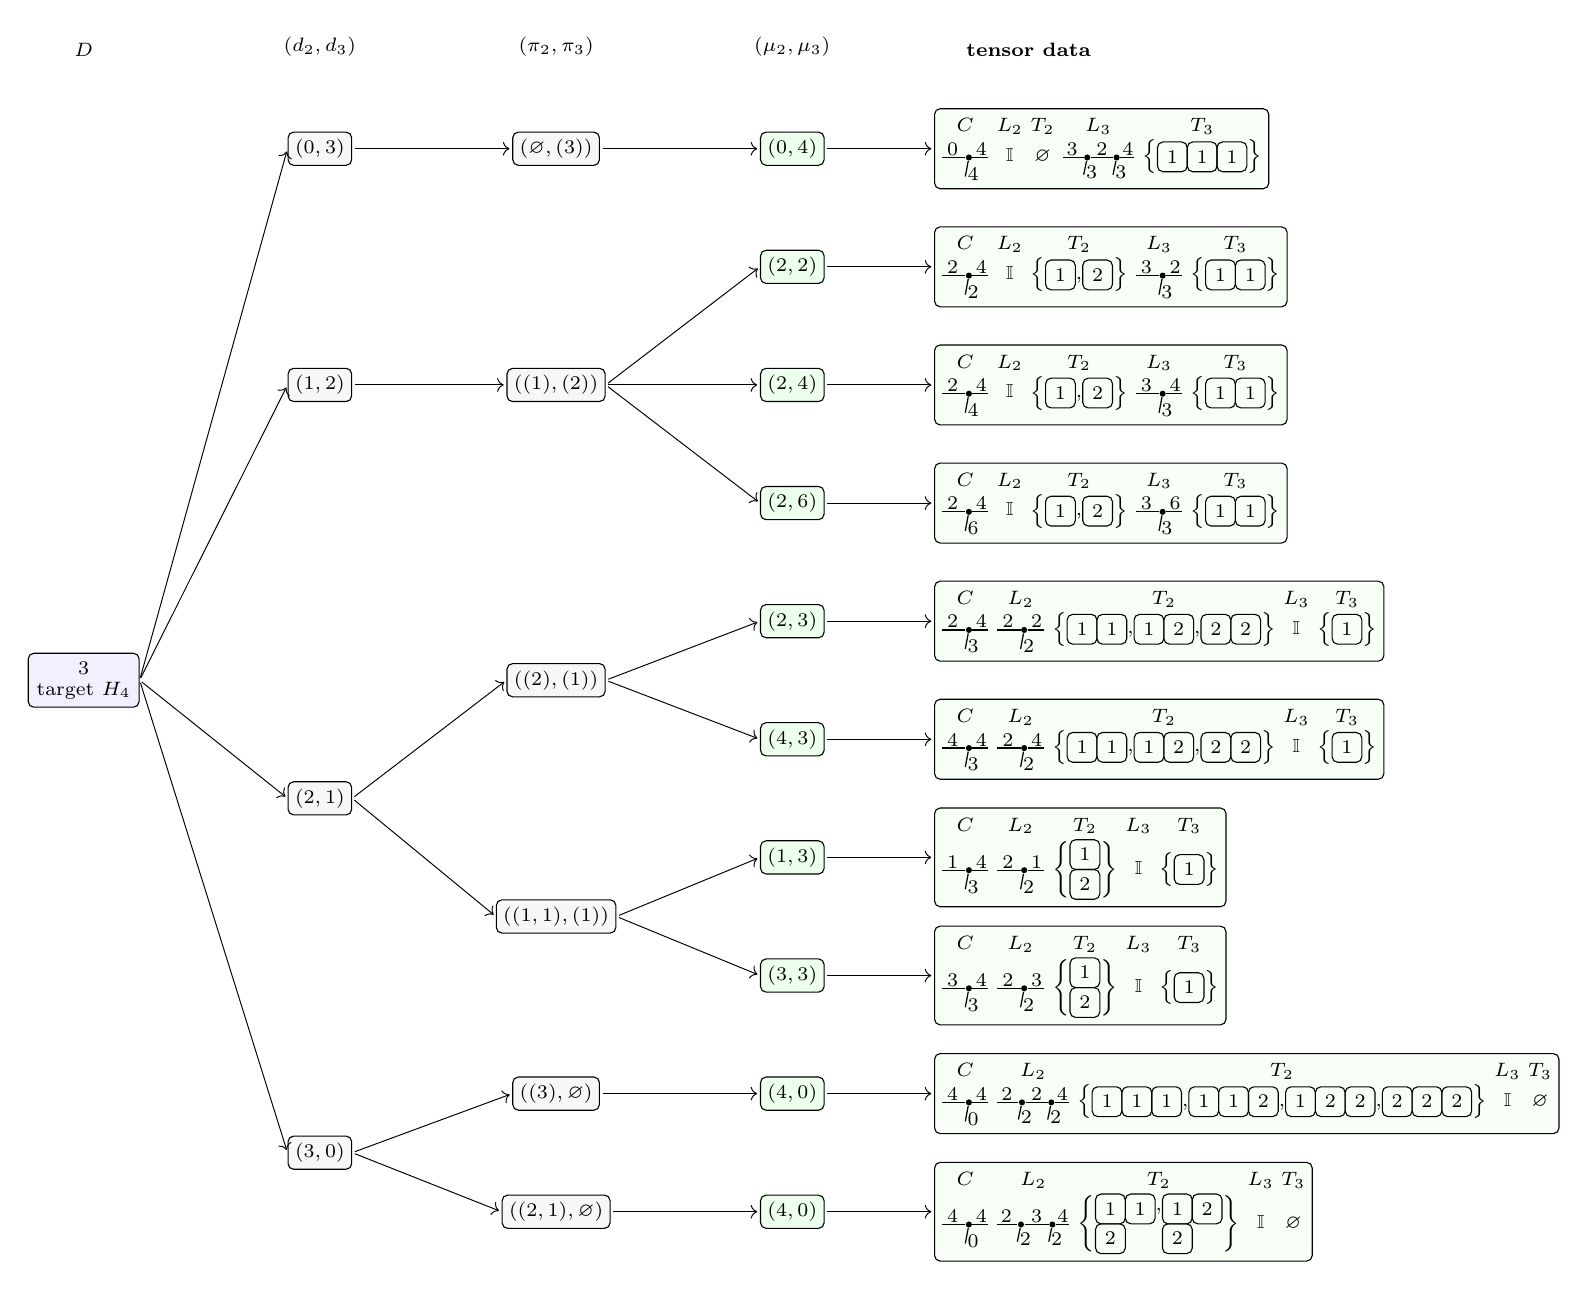
\begin{tikzpicture}[
        x=1.0cm,
        y=1.0cm,
        treeedge/.style={->, line width=0.35pt, shorten >=1pt, shorten <=1pt},
        root/.style={draw, rounded corners=2pt, align=center, fill=blue!6, inner sep=3pt},
        branch/.style={draw, rounded corners=2pt, align=center, fill=black!3, inner sep=2.5pt},
        mu/.style={draw, rounded corners=2pt, align=center, fill=green!7, inner sep=2.5pt},
        data/.style={draw, rounded corners=2pt, align=center, fill=green!3, inner sep=2.5pt, anchor=west},
        layerlabel/.style={font=\fontsize{6.8}{7.6}\selectfont\bfseries, anchor=south, align=center},
        every node/.style={font=\fontsize{6.8}{7.6}\selectfont}
      ]
        \node[layerlabel] at (0,1.05) {$D$};
        \node[root] (root) at (0,-6.75) {$3$\\target $H_4$};

        \node[layerlabel] at (3.0,1.05) {$(d_2,d_3)$};
        \node[branch] (d03) at (3.0,0) {$(0,3)$};
        \node[branch] (d12) at (3.0,-3.0) {$(1,2)$};
        \node[branch] (d21) at (3.0,-8.25) {$(2,1)$};
        \node[branch] (d30) at (3.0,-12.75) {$(3,0)$};

        \node[layerlabel] at (6.0,1.05) {$(\pi_2,\pi_3)$};
        \node[branch] (p03) at (6.0,0) {$(\varnothing,(3))$};
        \node[branch] (p12) at (6.0,-3.0) {$((1),(2))$};
        \node[branch] (p21s) at (6.0,-6.75) {$((2),(1))$};
        \node[branch] (p21a) at (6.0,-9.75) {$((1,1),(1))$};
        \node[branch] (p30s) at (6.0,-12.0) {$((3),\varnothing)$};
        \node[branch] (p30m) at (6.0,-13.5) {$((2,1),\varnothing)$};

        \node[layerlabel] at (9.0,1.05) {$(\mu_2,\mu_3)$};
        \node[mu] (m04) at (9.0,0) {$(0,4)$};
        \node[mu] (m22) at (9.0,-1.5) {$(2,2)$};
        \node[mu] (m24) at (9.0,-3.0) {$(2,4)$};
        \node[mu] (m26) at (9.0,-4.5) {$(2,6)$};
        \node[mu] (m23) at (9.0,-6.0) {$(2,3)$};
        \node[mu] (m43) at (9.0,-7.5) {$(4,3)$};
        \node[mu] (m13) at (9.0,-9.0) {$(1,3)$};
        \node[mu] (m33) at (9.0,-10.5) {$(3,3)$};
        \node[mu] (m40s) at (9.0,-12.0) {$(4,0)$};
        \node[mu] (m40m) at (9.0,-13.5) {$(4,0)$};

        \node[layerlabel] at (12.0,1.05) {tensor data};
        \node[data] (t04) at (10.8,0) {\IsoTensorData{\TTbin{0}{4}{4}}{\TTid}{\Yempty}{\TTtwo{3}{3}{2}{3}{4}}{\YDset{\Yrowthree{1}{1}{1}}}};
        \node[data] (t22) at (10.8,-1.5) {\IsoTensorData{\TTbin{2}{2}{4}}{\TTid}{\YDset{\Yone{1},\Yone{2}}}{\TTbin{3}{3}{2}}{\YDset{\Yrowtwo{1}{1}}}};
        \node[data] (t24) at (10.8,-3.0) {\IsoTensorData{\TTbin{2}{4}{4}}{\TTid}{\YDset{\Yone{1},\Yone{2}}}{\TTbin{3}{3}{4}}{\YDset{\Yrowtwo{1}{1}}}};
        \node[data] (t26) at (10.8,-4.5) {\IsoTensorData{\TTbin{2}{6}{4}}{\TTid}{\YDset{\Yone{1},\Yone{2}}}{\TTbin{3}{3}{6}}{\YDset{\Yrowtwo{1}{1}}}};
        \node[data] (t23) at (10.8,-6.0) {\IsoTensorData{\TTbin{2}{3}{4}}{\TTbin{2}{2}{2}}{\YDset{\Yrowtwo{1}{1},\Yrowtwo{1}{2},\Yrowtwo{2}{2}}}{\TTid}{\YDset{\Yone{1}}}};
        \node[data] (t43) at (10.8,-7.5) {\IsoTensorData{\TTbin{4}{3}{4}}{\TTbin{2}{2}{4}}{\YDset{\Yrowtwo{1}{1},\Yrowtwo{1}{2},\Yrowtwo{2}{2}}}{\TTid}{\YDset{\Yone{1}}}};
        \node[data] (t13) at (10.8,-9.0) {\IsoTensorData{\TTbin{1}{3}{4}}{\TTcolbin{2}{2}{1}}{\YDset{\Ycoltwo{1}{2}}}{\TTid}{\YDset{\Yone{1}}}};
        \node[data] (t33) at (10.8,-10.5) {\IsoTensorData{\TTbin{3}{3}{4}}{\TTcolbin{2}{2}{3}}{\YDset{\Ycoltwo{1}{2}}}{\TTid}{\YDset{\Yone{1}}}};
        \node[data] (t40s) at (10.8,-12.0) {\IsoTensorData{\TTbin{4}{0}{4}}{\TTtwo{2}{2}{2}{2}{4}}{\YDset{\Yrowthree{1}{1}{1},\Yrowthree{1}{1}{2},\Yrowthree{1}{2}{2},\Yrowthree{2}{2}{2}}}{\TTid}{\Yempty}};
        \node[data] (t40m) at (10.8,-13.5) {\IsoTensorData{\TTbin{4}{0}{4}}{\TThooktree{2}{2}{3}{2}{4}}{\YDset{\Yhook{1}{1}{2},\Yhook{1}{2}{2}}}{\TTid}{\Yempty}};

        \foreach \d in {d03,d12,d21,d30} {
          \draw[treeedge] (root.east) -- (\d.west);
        }
        \draw[treeedge] (d03.east) -- (p03.west);
        \draw[treeedge] (d12.east) -- (p12.west);
        \draw[treeedge] (d21.east) -- (p21s.west);
        \draw[treeedge] (d21.east) -- (p21a.west);
        \draw[treeedge] (d30.east) -- (p30s.west);
        \draw[treeedge] (d30.east) -- (p30m.west);

        \draw[treeedge] (p03.east) -- (m04.west);
        \draw[treeedge] (p12.east) -- (m22.west);
        \draw[treeedge] (p12.east) -- (m24.west);
        \draw[treeedge] (p12.east) -- (m26.west);
        \draw[treeedge] (p21s.east) -- (m23.west);
        \draw[treeedge] (p21s.east) -- (m43.west);
        \draw[treeedge] (p21a.east) -- (m13.west);
        \draw[treeedge] (p21a.east) -- (m33.west);
        \draw[treeedge] (p30s.east) -- (m40s.west);
        \draw[treeedge] (p30m.east) -- (m40m.west);

        \draw[treeedge] (m04.east) -- (t04.west);
        \draw[treeedge] (m22.east) -- (t22.west);
        \draw[treeedge] (m24.east) -- (t24.west);
        \draw[treeedge] (m26.east) -- (t26.west);
        \draw[treeedge] (m23.east) -- (t23.west);
        \draw[treeedge] (m43.east) -- (t43.west);
        \draw[treeedge] (m13.east) -- (t13.west);
        \draw[treeedge] (m33.east) -- (t33.west);
        \draw[treeedge] (m40s.east) -- (t40s.west);
        \draw[treeedge] (m40m.east) -- (t40m.west);
      \end{tikzpicture}%
    }
    \endgroup
    \caption{Condensed degree-$3$ isotypic data for $X=2H_2\oplus H_3$ and output $H_4$.}
    \label{fig:so3-degree-three-isotypic-tree}
  \end{figure}
\end{landscape}

\begin{example}[$\SO(3)$ Hilbert-series]\label{ex:so3-hilbert-shortcut}
  The specialized routine \texttt{hilbert\_series\_so3} computes
  \[
    \dim \scM_G^D(X,H_\nu)
    =
    \dim \HomG{H_\nu}{\scS^D(X)}
  \]
  from weight generating functions.
  If $X=\bigoplus_i H_{\lambda_i}^{\oplus m_i}$, then the weight generating function of $\scS(X)$ is
  \[
    \prod_i\prod_{w=-\lambda_i}^{\lambda_i}(1-tq^w)^{-m_i}.
  \]
  The coefficient of $t^Dq^m$ is the weight-$m$ multiplicity in $\scS^D(X)$, and the multiplicity of $H_\nu$ is the difference between the weight-$\nu$ and weight-$(\nu+1)$ multiplicities.
  This is an $\SO(3)$-specific fast path used to size random probe batches; the abstract algorithm can instead use the dimensions obtained directly from the constructed data trees.
\end{example}

\subsection{\texorpdfstring{$\Orth(3)$ from $\SO(3)$ parity}{O(3) from SO(3) parity}}\label{sec:examples-o3}

Let $z=-I$.
Since $\Orth(3)=\SO(3)\times \langle z\rangle$, every irreducible complex $\Orth(3)$-representation is a spin together with the scalar by which $z$ acts.
We write it as
\[
  H_\ell^\sigma,
  \qquad
  \ell\in\dsN_0,\quad \sigma\in\{\pm1\},
\]
where $H_\ell^\sigma|_{\SO(3)}=H_\ell$ and $z$ acts on $H_\ell^\sigma$ by $\sigma$.
Thus an $\Orth(3)$-representation has the parity-refined decomposition
\[
  X\cong
  \bigoplus_{\ell\ge 0}\bigoplus_{\sigma=\pm1}
  H_\ell^\sigma\otimes X_\ell^\sigma .
\]
If $X$ is first supplied only as an $\SO(3)$-module
\[
  X\cong \bigoplus_{\ell\ge 0} H_\ell\otimes X_\ell,
\]
then $X_\ell^\sigma$ is the $\sigma$-eigenspace for the action of $z$ on the multiplicity space $X_\ell$.
For example, if $z$ swaps two spin-$\ell$ copies $e_1,e_2\in X_\ell$, then replacing them by
\[
  e_+ = e_1+e_2,
  \qquad
  e_- = e_1-e_2
\]
gives the $+$ and $-$ parity copies.
Thus copy permutation by $-I$ is just the diagonalization step which produces the spaces $X_\ell^+$ and $X_\ell^-$.

\subsubsection{Parity-refined \texorpdfstring{$\SO(3)$}{SO(3)} data}

The $\Orth(3)$ Clebsch--Gordan rule is the $\SO(3)$ rule with parities multiplied:
\[
  H_{\ell_1}^{\sigma_1}\otimes H_{\ell_2}^{\sigma_2}
  \cong
  \bigoplus_{\nu=|\ell_1-\ell_2|}^{\ell_1+\ell_2}
  H_\nu^{\sigma_1\sigma_2}.
\]
The Schur-power multiplicities are also the same as in Eq.~\eqref{eq:so3-schur-multiplicity}; only the parity label changes:
\[
  \operatorname{Hom}_{\Orth(3)}\!\left(
    H_\mu^{\sigma^d},
    e_\pi\!\left((H_\ell^\sigma)^{\otimes d}\right)
  \right)
  \cong
  \operatorname{Hom}_{\SO(3)}\!\left(
    H_\mu,
    e_\pi(H_\ell^{\otimes d})
  \right),
\]
and no other output parity occurs.

Consequently, Theorem~\ref{thm:isotypic-decomposition} applies to $\Orth(3)$ by using the labels $(\ell,\sigma)$ instead of the labels $\ell$.
A branch choosing $d_{\ell,\sigma}$ inputs from $H_\ell^\sigma\otimes X_\ell^\sigma$ has central parity
\[
  \prod_{\ell,\sigma}\sigma^{d_{\ell,\sigma}}.
\]
It can contribute to an output $H_\nu^\tau$ only when this product equals $\tau$.
This parity selection rule is the only change from the $\SO(3)$ data tree.

\subsubsection{\texorpdfstring{$\Orth(3)$-equivariant covariants}{O(3)-equivariant covariants}}

For an output representation
\[
  Y\cong
  \bigoplus_{\nu\ge 0}\bigoplus_{\tau=\pm1}
  H_\nu^\tau\otimes Y_\nu^\tau,
\]
the usual output reduction becomes
\[
  \scM_{\Orth(3)}^D(X,Y)
  \cong
  \bigoplus_{\nu,\tau}
  \operatorname{Hom}_{\Orth(3)}\!\left(H_\nu^\tau,\scS^D(X)\right)^*
  \otimes Y_\nu^\tau .
\]
Equivalently, compute the $\SO(3)$ branches as before, attach to each branch its input parity, and keep only the branches whose input parity is $\tau$ for the output copy $Y_\nu^\tau$.
In particular,
\[
  \scM_{\Orth(3)}^D(X,H_\nu^\tau)
  \cong
  \operatorname{Hom}_{\Orth(3)}\!\left(H_\nu^\tau,\scS^D(X)\right)^*,
\]
where the right-hand side is obtained from the spin-$\nu$ $\SO(3)$ multiplicity space by the same parity filter.

\subsubsection{Even, odd, and pseudoscalar generators}

The central element acts on $\SO(3)$-covariants by
\[
  (z\cdot f)(x)=z\,f(z^{-1}x),
\]
where $z$ acts on $X$ in the argument and on $Y$ in the value.
A covariant is even or odd according as $z\cdot f=f$ or $z\cdot f=-f$.
The $\Orth(3)$-equivariant covariants are exactly the even $\SO(3)$-covariants:
\[
  \scM_{\Orth(3)}^D(X,Y)
  =
  \left(\scM_{\SO(3)}^D(X,Y)\right)^z .
\]

For scalar invariants, $z$ acts trivially on the value, so a scalar $f$ has parity $\sigma$ precisely when
\[
  f(zx)=\sigma f(x).
\]
Hence
\[
  \scR_{\Orth(3)}^D(X)
  =
  \left(\scR_{\SO(3)}^D(X)\right)^z
  =
  \scR_{\SO(3),+}^D(X).
\]
The odd scalar $\SO(3)$-invariants are pseudoscalars: they change sign under central inversion and therefore are not $\Orth(3)$-invariants.

Thus the generator computation needs no separate $\Orth(3)$ machinery.
Use the $\SO(3)$ candidate branches, record the product of the input parities, and keep even scalar generators for $\scR_{\Orth(3)}(X)$ or parity-$\tau$ covariant generators for an output copy $H_\nu^\tau$.

\subsection{\texorpdfstring{$G\times K$}{G x K}}\label{sec:examples-g-times-k}

A useful product-group example is obtained by adding copy permutation symmetry to the $G$-action.
Assume that, in the isotypic decomposition
\[
  X\cong\bigoplus_\lambda H_\lambda\otimes X_\lambda,
\]
each multiplicity space is the permutation representation of $\mathfrak S_{m_\lambda}$:
\[
  X_\lambda\cong \dsC^{m_\lambda}
  \cong
  \mathbf{1}_\lambda\oplus \operatorname{Std}_\lambda,
\]
where $\mathfrak S_{m_\lambda}$ permutes the standard basis of $\dsC^{m_\lambda}$.
Set
\[
  K\coloneq \prod_\lambda \mathfrak S_{m_\lambda}.
\]
For $\sigma=(\sigma_\lambda)_\lambda\in K$, define
\[
  \sigma\cdot(h\otimes x_\lambda)
  =
  h\otimes (\sigma_\lambda x_\lambda),
  \qquad
  h\in H_\lambda,\quad x_\lambda\in X_\lambda.
\]
This action commutes with $G$, since $G$ acts only on the $H_\lambda$-factors, and hence defines an action of $G\times K$ on $X$.

Equip $H_\nu$ with the trivial $K$-action.
On the Hom side of the construction, imposing copy permutation equivariance means taking
\[
  \operatorname{Hom}_{G\times K}\!\left(H_\nu,\scS^D(X)\right)
  =
  \HomG{H_\nu}{\scS^D(X)}^K.
\]
In each summand of Eq.~\eqref{eq:isotypic-decomposition}, $K$ acts trivially on
\[
  \HomG{H_\nu}{\bigotimes_\lambda H_{\mu_\lambda}},
  \qquad
  \HomG{H_{\mu_\lambda}}{e_{\pi_\lambda}(H_\lambda^{\otimes d_\lambda})},
\]
so the only change is on the Schur-side multiplicity factor:
\[
  \bigotimes_\lambda e_{\pi_\lambda}^*(X_\lambda^{\otimes d_\lambda})
  \quad\leadsto\quad
  \bigotimes_\lambda
  \left(e_{\pi_\lambda}^*(X_\lambda^{\otimes d_\lambda})\right)^{\mathfrak S_{m_\lambda}}.
\]
Equivalently, for each $\lambda$ project by
\[
  \frac{1}{m_\lambda!}
  \sum_{\sigma\in\mathfrak S_{m_\lambda}}
  \sigma^{\otimes d_\lambda}
  :
  e_{\pi_\lambda}^*(X_\lambda^{\otimes d_\lambda})
  \longrightarrow
  e_{\pi_\lambda}^*(X_\lambda^{\otimes d_\lambda}).
\]
Here $\sigma^{\otimes d_\lambda}$ preserves the Schur-side factor.
It commutes with the place-permutation action used to define $e_{\pi_\lambda}^*$.
Thus the ordinary isotypic data tree is unchanged; only the tableau-tensor basis for each $\lambda$ is replaced by a basis of
\[
  \left(e_{\pi_\lambda}^*(X_\lambda^{\otimes d_\lambda})\right)^{\mathfrak S_{m_\lambda}}.
\]

\section{Conclusion}\label{sec:conclusion}

Several questions remain for future work:
\begin{itemize}[leftmargin=2em]
  \item Do the sequences $\{\dim \scR_G^D(X)\}_{D \in \dsN_0}$ and $\{\dim \scM_G^D(X,Y)\}_{D \in \dsN_0}$ appear in the OEIS?
  What connections can be made?
  \item Would the evaluation stage perform better if one replaced the CP decomposition of partially symmetrized monomials by the standard polarization identity for symmetric multilinear forms \cite[Theorem~1 and Eq.~(7)]{Thomas2014}?
  \item What is the precise role of semistandard Young tableaux in the final generator sets?
  Can algebraic or module redundancy already be detected from the spin-coupling trees before tableau data are assembled?
  \item More specifically, any spin tree with a vanishing interior spin corresponds to a product of lower-degree invariants and covariants.
  Can this observation be incorporated directly into the tree-construction stage to prune redundant branches earlier?
\end{itemize}

\begin{thebibliography}{99}

  \bibitem{FH1991}
  W.~Fulton and J.~Harris,
  \emph{Representation Theory: A First Course},
  Graduate Texts in Mathematics 129,
  Springer, 1991.

  \bibitem{GW2009}
  R.~Goodman and N.~R.~Wallach,
  \emph{Symmetry, Representations, and Invariants},
  Graduate Texts in Mathematics 255,
  Springer, 2009.

  \bibitem{BK2001}
  B.~Bakalov and A.~Kirillov Jr.,
  \emph{Lectures on Tensor Categories and Modular Functors},
  University Lecture Series 21,
  American Mathematical Society, 2001.

  \bibitem{Sellerstam2019}
  O.~Sellerstam,
  \emph{Representations of $\SO(3)$ in $\dsC[x,y,z]$},
  Degree project in technology, KTH Royal Institute of Technology, 2019.

  \bibitem{Weyman2003}
  J.~Weyman,
  \emph{Cohomology of Vector Bundles and Syzygies},
  Cambridge Tracts in Mathematics 149,
  Cambridge University Press, 2003.

  \bibitem{BBT2013}
  W.~Buczy\'nska, J.~Buczy\'nski, and Z.~Teitler,
  Waring decompositions of monomials,
  \emph{Journal of Algebra} 378 (2013), 45--57.

  \bibitem{Sturmfels2008}
  B.~Sturmfels,
  \emph{Algorithms in Invariant Theory},
  2nd ed.,
  Texts \& Monographs in Symbolic Computation,
  Springer Vienna, 2008.

  \bibitem{OKA2017}
  M.~Olive, B.~Kolev, and N.~Auffray,
  A minimal integrity basis for the elasticity tensor,
  \emph{Archive for Rational Mechanics and Analysis} 226 (2017), 1--31.

  \bibitem{Olive2017}
  M.~Olive,
  About Gordan's algorithm for binary forms,
  \emph{Foundations of Computational Mathematics} 17 (2017), 1407--1466.

  \bibitem{Bourbaki1989}
  N.~Bourbaki,
  \emph{Algebra I: Chapters 1--3},
  Elements of Mathematics,
  Springer, 1989.

  \bibitem{Springer1977}
  T.~A.~Springer,
  \emph{Invariant Theory},
  Lecture Notes in Mathematics 585,
  Springer, 1977.

  \bibitem{DCP2021}
  G.~Dhont, P.~Cassam-Chena\"i, and F.~Patras,
  Molien generating functions and integrity bases for the action of the $\SO(3)$ and $\Orth(3)$ groups on a set of vectors,
  \emph{arXiv preprint} arXiv:1511.01311v3, 2021.

  \bibitem{Schwartz1980}
  J.~T.~Schwartz,
  Fast probabilistic algorithms for verification of polynomial identities,
  \emph{Journal of the ACM} 27 (1980), no.~4, 701--717.

  \bibitem{Zippel1979}
  R.~Zippel,
  Probabilistic algorithms for sparse polynomials,
  in \emph{Symbolic and Algebraic Computation: EUROSAM '79},
  Lecture Notes in Computer Science 72,
  Springer, 1979, pp.~216--226.


  \bibitem{Stacks0EKB}
  The Stacks Project Authors,
  \emph{The Stacks Project},
  \href{https://stacks.math.columbia.edu/tag/0EKB}{Tag 0EKB}.

  \bibitem{Thomas2014}
  E.~G.~F.~Thomas,
  A polarization identity for multilinear maps,
  \emph{Indagationes Mathematicae} (N.S.) 25 (2014), no.~3, 468--474.

  \bibitem{Gregory2024}
  W.~G.~Gregory, J.~Tonelli-Cueto, N.~F.~Marshall, A.~S.~Lee, and S.~Villar,
  Tensor learning with orthogonal, Lorentz, and symplectic symmetries,
  \emph{arXiv preprint} arXiv:2406.01552, 2024; published as a conference paper at ICLR 2026.

  \bibitem{BlumSmithVillar2023}
  B.~Blum-Smith and S.~Villar,
  Machine learning and invariant theory,
  \emph{Notices of the American Mathematical Society} 70 (2023), no.~8, 1205--1213.

  \bibitem{Pinkus1999}
  A.~Pinkus,
  Approximation theory of the MLP model in neural networks,
  \emph{Acta Numerica} 8 (1999), 143--195.

  \bibitem{LeshnoLinPinkusSchocken1993}
  M.~Leshno, V.~Ya.~Lin, A.~Pinkus, and S.~Schocken,
  Multilayer feedforward networks with a nonpolynomial activation function can approximate any function,
  \emph{Neural Networks} 6 (1993), no.~6, 861--867.


  \bibitem{cohen2016gcnn}
  T.~S.~Cohen and M.~Welling,
  Group equivariant convolutional networks,
  in \emph{Proceedings of the 33rd International Conference on Machine Learning},
  PMLR 48, 2016.

  \bibitem{finzi2021emlp}
  M.~Finzi, M.~Welling, and A.~G.~Wilson,
  A practical method for constructing equivariant multilayer perceptrons for arbitrary matrix groups,
  in \emph{Proceedings of the 38th International Conference on Machine Learning},
  PMLR 139, 2021.

  \bibitem{Thomas2018tfn}
  N.~Thomas, T.~Smidt, S.~Kearnes, L.~Yang, L.~Li, K.~Kohlhoff, and P.~Riley,
  Tensor field networks: Rotation- and translation-equivariant neural networks for 3D point clouds,
  \emph{arXiv preprint} arXiv:1802.08219, 2018.

  \bibitem{kondor2018cgnets}
  R.~Kondor, Z.~Lin, and S.~Trivedi,
  Clebsch--Gordan nets: A fully Fourier space spherical convolutional neural network,
  in \emph{Advances in Neural Information Processing Systems}, 2018.

  \bibitem{Kamnitzer2011}
  J.~Kamnitzer,
  \emph{Representation Theory of Compact Groups and Complex Semisimple Lie Groups},
  course notes, University of Toronto, 2011.

  \bibitem{BR2008}
  J.~Brunnemann and D.~Rideout,
  Properties of the volume operator in loop quantum gravity II: detailed presentation,
  \emph{Classical and Quantum Gravity} 25 (2008), 065002.

  \bibitem{Derksen1999}
  H.~Derksen,
  Computation of invariants for reductive groups,
  \emph{Advances in Mathematics} 141 (1999), no.~2, 366--384.

  \bibitem{DerksenKemper2002}
  H.~Derksen and G.~Kemper,
  \emph{Computational Invariant Theory},
  Encyclopaedia of Mathematical Sciences 130,
  Springer, 2002.

\end{thebibliography}

\appendix

\section{Proofs}\label{sec:appendix-proofs}

\subsection{Preliminary results}


\begin{proposition}[Isotypic decomposition]\label{prop:isotypic-decomposition}
  Let $V$ be a finite-dimensional $G$-representation.
  There is a $G$-equivariant isomorphism
  \[
    V
    \cong
    \bigoplus_{\lambda}
    H_\lambda\otimes \HomG{H_\lambda}{V},
  \]
  where $G$ acts trivially on each multiplicity space $\HomG{H_\lambda}{V}$.
  Moreover, the isomorphism (from right to left) is the evaluation map
  \[
    \bigoplus_{\lambda}
    H_\lambda\otimes \HomG{H_\lambda}{V}
    \longrightarrow
    V,
    \quad
    v\otimes \varphi \longmapsto \varphi(v).
  \]
\end{proposition}
\begin{proof}
  See Kamnitzer~\cite[Theorem~1.10 and its proof]{Kamnitzer2011}.
\end{proof}

\begin{proposition}[Symmetric power of a finite direct sum]\label{prop:sym-direct-sum}
  Let $\{V_\lambda\}_\lambda$ be a finite collection of $G$-representations, and let $D\in\dsN_0$.
  There is a $G$-equivariant isomorphism
  \[
    \scS^D\!\left(\bigoplus_\lambda V_\lambda\right)
    \cong
    \bigoplus_{(d_\lambda)_\lambda}\bigotimes_\lambda \scS^{d_\lambda}(V_\lambda),
  \]
  where $(d_\lambda)_\lambda$ ranges over all sequences of nonnegative integers such that $\sum_\lambda d_\lambda=D$.
  Moreover, the isomorphism (from right to left) is given by symmetrization over the $D$ tensor factors.
\end{proposition}
\begin{proof}
  This is the degree-$D$ piece of the graded algebra isomorphism
  \[
    \scS\!\left(\bigoplus_\lambda V_\lambda\right)
    \cong
    \bigotimes_\lambda \scS(V_\lambda).
  \]
  See Bourbaki~\cite[Chapter III, \S6.6, Proposition 9]{Bourbaki1989}.
\end{proof}

\begin{definition}[Young symmetrizer]\label{def:young-symmetrizer}
  Let $\pi$ be a partition of $d$, let $T_\pi$ be the row--ordered standard Young tableau of shape $\pi$, and let $R_\pi,C_\pi\subset \mathfrak{S}_d$ be its row and column stabilizers.
  The \emph{row}, \emph{column}, and \emph{Young symmetrizers} are
  \[
    r_\pi\coloneq \frac{1}{|R_\pi|}\sum_{\sigma\in R_\pi}\sigma,
    \quad
    c_\pi\coloneq \frac{1}{|C_\pi|}\sum_{\sigma\in C_\pi}\operatorname{sgn}(\sigma)\sigma,
    \quad
    e_\pi\coloneq \frac{|R_\pi||C_\pi|}{\mathrm{HL}_\pi}\,r_\pi c_\pi
  \]
  respectively, where $\mathrm{HL}_\pi$ is the hook-length product.
  Note that the Young symmetrizer $e_\pi$ is an idempotent in $\dsR[\mathfrak{S}_d]$.
\end{definition}

\begin{theorem}[Cauchy decomposition]\label{thm:cauchy}
  Let $V$ and $W$ be finite-dimensional complex vector spaces, and let $d \in \dsN_0$.
  There is a $\GL(V)\times \GL(W)$-equivariant isomorphism
  \begin{equation}\label{eq:cauchy}
    \scS^d(V\otimes W)
    \cong
    \bigoplus_\pi
    e_\pi(V^{\otimes d})\otimes e_\pi^*(W^{\otimes d}),
  \end{equation}
  where the sum is over all integer partitions $\pi\vdash d$ with at most $\min(\dim V,\dim W)$ parts.
  Moreover, the isomorphism (from right to left) is given by rearranging the tensor product and symmetrizing.
\end{theorem}
\begin{proof}
  See Weyman~\cite[\S2.3, Corollary 2.3.3]{Weyman2003}.
\end{proof}

\begin{lemma}[Transfer identity]\label{lem:cauchy-transfer}
  Let $V$ and $W$ be vector spaces, let $d\in\dsN_0$, and let
  \[
    \tau:V^{\otimes d}\otimes W^{\otimes d}\longrightarrow (V\otimes W)^{\otimes d}
  \]
  be the natural reshuffling isomorphism.
  Let
  \[
    P_d=\frac{1}{d!}\sum_{\sigma\in\mathfrak S_d}\sigma
  \]
  be the symmetrizer on $(V\otimes W)^{\otimes d}$.
  Then for any $e\in \dsR[\mathfrak S_d]$,
  \[
    P_d\tau(1\otimes e^*)
    =
    P_d\tau(e\otimes 1).
  \]
\end{lemma}
\begin{proof}
  Under $\tau$, the symmetrizer $P_d$ becomes the diagonal operator
  \[
    P_d\tau=\frac{1}{d!}\sum_{\sigma\in\mathfrak S_d}\sigma\otimes\sigma
  \]
  on $V^{\otimes d}\otimes W^{\otimes d}$.
  Thus, for any
  \[
    e=\sum_{\rho\in\mathfrak S_d} e_\rho\,\rho \in \dsC[\mathfrak S_d],
  \]
  we have
  \[
    P_d\tau(1\otimes e^*)
    =
    \frac{1}{d!}\sum_{\sigma,\rho} e_\rho\,\sigma\otimes \sigma\rho^*
    =
    \frac{1}{d!}\sum_{\sigma,\rho} e_\rho\,\sigma\rho\otimes \sigma
    =
    P_d\tau(e\otimes 1),
  \]
  where we reindexed $\sigma\mapsto \sigma\rho$.
\end{proof}

\subsection{Proof of Theorem~\ref{thm:isotypic-decomposition}}\label{sec:proof-main-decomposition}

Because $X$ is finite dimensional, only finitely many $\lambda$ satisfy $X_\lambda\neq 0$.
Applying Proposition~\ref{prop:sym-direct-sum} to the isotypic decomposition of $X$, we have
\[
  \scS^D(X)
  \cong
  \scS^D\!\left(\bigoplus_\lambda H_\lambda\otimes X_\lambda\right)
  \cong
  \bigoplus_{(d_\lambda)_\lambda}
  \bigotimes_\lambda
  \scS^{d_\lambda}(H_\lambda\otimes X_\lambda),
\]
where $(d_\lambda)_\lambda$ ranges over all sequences of nonnegative integers such that $\sum_\lambda d_\lambda=D$.
For each $\lambda$, Theorem~\ref{thm:cauchy} gives
\[
  \scS^{d_\lambda}(H_\lambda\otimes X_\lambda)
  \cong
  \bigoplus_{\pi_\lambda}
  e_{\pi_\lambda}(H_\lambda^{\otimes d_\lambda})\otimes e_{\pi_\lambda}^*(X_\lambda^{\otimes d_\lambda}),
\]
where $\pi_\lambda$ ranges over all partitions of $d_\lambda$ with at most $\min(\dim H_\lambda,\dim X_\lambda)$ parts.
Substituting this into the previous display gives
\[
  \scS^D(X)
  \cong
  \bigoplus_{(d_\lambda)_\lambda}
  \bigotimes_\lambda
  \left(
  \bigoplus_{\pi_\lambda}
  e_{\pi_\lambda}(H_\lambda^{\otimes d_\lambda})\otimes e_{\pi_\lambda}^*(X_\lambda^{\otimes d_\lambda})
  \right).
\]
Since only finitely many $\lambda$ occur, we may distribute the tensor product over the direct sum and rearrange the tensor product to obtain
\[
  \scS^D(X)
  \cong
  \bigoplus_{(d_\lambda)_\lambda}
  \bigoplus_{(\pi_\lambda)_\lambda}
  \left(\bigotimes_\lambda e_{\pi_\lambda}(H_\lambda^{\otimes d_\lambda})\right)
  \otimes
  \left(\bigotimes_\lambda e_{\pi_\lambda}^*(X_\lambda^{\otimes d_\lambda})\right).
\]
Now, for each $\lambda$, take the isotypic decomposition
\[
  e_{\pi_\lambda}(H_\lambda^{\otimes d_\lambda})
  \cong
  \bigoplus_{\mu_\lambda}
  H_{\mu_\lambda}\otimes \HomG{H_{\mu_\lambda}}{e_{\pi_\lambda}(H_\lambda^{\otimes d_\lambda})},
\]
where $\mu_\lambda$ ranges over all nonnegative integers such that
\[
  \HomG{H_{\mu_\lambda}}{e_{\pi_\lambda}(H_\lambda^{\otimes d_\lambda})}\neq 0.
\]
Substituting gives
\[
  \scS^D(X)
  \cong
  \bigoplus_{(d_\lambda)_\lambda}
  \bigoplus_{(\pi_\lambda)_\lambda}
  \left(\bigotimes_\lambda
  \left(
  \bigoplus_{\mu_\lambda}
  H_{\mu_\lambda}\otimes \HomG{H_{\mu_\lambda}}{e_{\pi_\lambda}(H_\lambda^{\otimes d_\lambda})}
  \right)\right)
  \otimes
  \left(\bigotimes_\lambda e_{\pi_\lambda}^*(X_\lambda^{\otimes d_\lambda})\right).
\]
Again distributing the tensor product over the direct sum and rearranging the tensor product, we obtain
\[
  \scS^D(X)
  \cong
  \bigoplus_{(d_\lambda)_\lambda}
  \bigoplus_{(\pi_\lambda)_\lambda}
  \bigoplus_{(\mu_\lambda)_\lambda}
  \left(\bigotimes_\lambda H_{\mu_\lambda}\right)
  \otimes
  \left(\bigotimes_\lambda \HomG{H_{\mu_\lambda}}{e_{\pi_\lambda}(H_\lambda^{\otimes d_\lambda})}\right)
  \otimes
  \left(\bigotimes_\lambda e_{\pi_\lambda}^*(X_\lambda^{\otimes d_\lambda})\right),
\]
where $(\mu_\lambda)_\lambda$ ranges over all sequences of nonnegative integers such that
\[
  \HomG{H_{\mu_\lambda}}{e_{\pi_\lambda}(H_\lambda^{\otimes d_\lambda})}\neq 0
\]
for all $\lambda$.
Finally, apply $\HomG{H_\nu}{-}$ to both sides.
Since $\HomG{H_\nu}{-}$ preserves finite direct sums, and since each space
\[
  \HomG{H_{\mu_\lambda}}{e_{\pi_\lambda}(H_\lambda^{\otimes d_\lambda})}
  \quad\text{and}\quad
  e_{\pi_\lambda}^*(X_\lambda^{\otimes d_\lambda})
\]
carries the trivial $G$-action, we have
\begin{align*}
  \HomG{H_\nu}{\scS^D(X)}
  &\cong
  \bigoplus_{(d_\lambda)_\lambda}
  \bigoplus_{(\pi_\lambda)_\lambda}
  \bigoplus_{(\mu_\lambda)_\lambda}
  \HomG{H_\nu}{\bigotimes_\lambda H_{\mu_\lambda}}\otimes\\
  &\qquad
  \bigotimes_\lambda
  \HomG{H_{\mu_\lambda}}{e_{\pi_\lambda}(H_\lambda^{\otimes d_\lambda})}
  \otimes
  \bigotimes_\lambda e_{\pi_\lambda}^*(X_\lambda^{\otimes d_\lambda}).
\end{align*}
Restricting to those $(\mu_\lambda)_\lambda$ for which
\[
  \HomG{H_\nu}{\bigotimes_\lambda H_{\mu_\lambda}}\neq 0
\]
does not change the direct sum, and we are done.

\subsection{Proof of Theorem~\ref{thm:evaluation}}\label{sec:proof-evaluation}
Following the proof of Theorem~\ref{thm:isotypic-decomposition} in reverse, the isomorphism in Eq.~\eqref{eq:isotypic-decomposition} acts on the elementary tensor in Eq.~\eqref{eq:isotypic-data-tensor} as follows.
First, compose the core tensor $C$ with the Young-symmetrized leaf tensors $e_{\pi_\lambda} L_\lambda$ in each mode to obtain
\[
  \left(\bigotimes_\lambda e_{\pi_\lambda} L_\lambda\right)
  \circ
  C
  \in \HomG{H_\nu}{\bigotimes_\lambda e_{\pi_\lambda}(H_\lambda^{\otimes d_\lambda})}.
\]
Next, take the tensor product with the Young-symmetrized tableau tensors $e_{\pi_\lambda}^*T_\lambda$ and rearrange the tensor product to obtain
\[
  \left(\id \otimes \left(\bigotimes_\lambda e_{\pi_\lambda}^*T_\lambda\right)\right)
  \circ
  \left(\bigotimes_\lambda e_{\pi_\lambda} L_\lambda\right)
  \circ
  C
  \in \HomG{H_\nu}{\bigotimes_\lambda e_{\pi_\lambda}(H_\lambda^{\otimes d_\lambda})
  \otimes
  e_{\pi_\lambda}^*(X_\lambda^{\otimes d_\lambda})}.
\]
Then, for each $\lambda$, apply the inverse Cauchy map
\[
  P_{d_\lambda}\tau:
  e_{\pi_\lambda}(H_\lambda^{\otimes d_\lambda})\otimes e_{\pi_\lambda}^*(X_\lambda^{\otimes d_\lambda})
  \longrightarrow
  \scS^{d_\lambda}(H_\lambda\otimes X_\lambda)
\]
as in Lemma \ref{lem:cauchy-transfer} and symmetrize across all $D$ factors as in Proposition \ref{prop:sym-direct-sum} to obtain
\[
  \Sym
  \circ
  \left(\bigotimes_\lambda P_{d_\lambda}\tau\right)
  \circ
  \left(\id \otimes \left(\bigotimes_\lambda e_{\pi_\lambda}^*T_\lambda\right)\right)
  \circ
  \left(\bigotimes_\lambda e_{\pi_\lambda} L_\lambda\right)
  \circ
  C
  \in \HomG{H_\nu}{\scS^D(X)}.
\]
Now, by Lemma \ref{lem:cauchy-transfer}, for every $z\in H_{\mu_\lambda}$,
\begin{align*}
  P_{d_\lambda}\tau\Bigl((e_{\pi_\lambda}L_\lambda)(z)\otimes e_{\pi_\lambda}^*T_\lambda\Bigr)
  &=
  P_{d_\lambda}\tau\Bigl((e_{\pi_\lambda}e_{\pi_\lambda}L_\lambda)(z)\otimes T_\lambda\Bigr) \\
  &=
  P_{d_\lambda}\tau\Bigl((e_{\pi_\lambda}L_\lambda)(z)\otimes T_\lambda\Bigr).
\end{align*}
Thus the factors $e_{\pi_\lambda}^*$ acting on $T_\lambda$ can be removed.
To complete the proof, recall that
\[
  X_\lambda = \HomG{H_\lambda}{X}.
\]
Thus, every tableau tensor $T_\lambda\in X_\lambda^{\otimes d_\lambda}$ can be viewed as a linear map $T_\lambda \in \HomG{H_\lambda^{\otimes d_\lambda}}{X^{\otimes d_\lambda}}$.
With this identification, we have
\[
  \tau(u\otimes T_\lambda)=T_\lambda(u)
  \quad
  \text{for all}
  \quad
  u\in H_\lambda^{\otimes d_\lambda}
\]
up to the isomorphism in Proposition \ref{prop:isotypic-decomposition}.
Substituting this yields
\[
  p
  =
  \Sym
  \circ
  \left(\bigotimes_\lambda P_{d_\lambda}\circ T_\lambda\right)
  \circ
  \left(\bigotimes_\lambda e_{\pi_\lambda}L_\lambda\right)
  \circ
  C.
\]
Absorbing the symmetrizers $P_{d_\lambda}$ into the full symmetrizer $\Sym$ yields
\[
  \Sym
  \circ
  \left(\bigotimes_\lambda P_{d_\lambda}\circ T_\lambda\right)
  =
  \Sym
  \circ
  \left(\bigotimes_\lambda T_\lambda\right).
\]
Substituting this identity proves Eq.~\eqref{eq:evaluation}.

\subsection{Proof of Corollary~\ref{cor:evaluation}}\label{sec:proof-corollary-evaluation}

Fix $x\in X$ and $y\in H_\nu$.
By Theorem~\ref{thm:evaluation},
\[
  p
  =
  \Sym
  \circ
  \left(\bigotimes_\lambda T_\lambda\right)
  \circ
  \left(\bigotimes_\lambda e_{\pi_\lambda}L_\lambda\right)
  \circ
  C.
\]
Thus,
\begin{align*}
  \langle p^*(x),y\rangle
  &=
  \langle x^{\otimes D},p(y)\rangle \\
  &=
  \left\langle
  x^{\otimes D},
  \Sym
  \circ
  \left(\bigotimes_\lambda T_\lambda\right)
  \circ
  \left(\bigotimes_\lambda e_{\pi_\lambda}L_\lambda\right)
  \circ
  C(y)
  \right\rangle \\
  &=
  \left\langle
  \bigotimes_\lambda x^{\otimes d_\lambda},
  \left(\bigotimes_\lambda T_\lambda\right)
  \circ
  \left(\bigotimes_\lambda e_{\pi_\lambda}L_\lambda\right)
  \circ
  C(y)
  \right\rangle \\
  &=
  \left\langle
  C^*
  \circ
  \left(\bigotimes_\lambda L_\lambda^*e_{\pi_\lambda}^*\right)
  \circ
  \left(\bigotimes_\lambda T_\lambda^*(x^{\otimes d_\lambda})\right),
  y
  \right\rangle.
\end{align*}
Since this holds for all $y\in H_\nu$, the stated formula follows.

\section{Implementation details}
\label{sec:appendix-implementation}

\subsection{Evaluation and rank extraction}

\begin{proposition}[Finite-field rank extraction by random evaluation]\label{prop:random-rank-test}
  Let $f_1,\dots,f_N$ be polynomial maps $\dsF_p^n\to\dsF_p^q$ of degree at most $D$, and let $Z=(z^{(1)},\dots,z^{(m)})$ denote $m$ formal probes in $\dsF_p^n$.
  Form the stacked evaluation matrix
  \[
    E(Z)\in \operatorname{Mat}_{mq\times N}\left(\dsF_p[Z]\right)
  \]
  whose $j$-th column stacks $f_j(z^{(1)}),\dots,f_j(z^{(m)})$.
  Suppose that the column span of $E(Z)$ has rank $r$ over the function field $\dsF_p(Z)$, equivalently that some $r\times r$ minor $\Delta(Z)$ is a nonzero polynomial.
  If the coordinates of $Z$ are sampled independently and uniformly from $\dsF_p$, then
  \[
    \Pr\left[\operatorname{rank}_{\dsF_p}E(Z)<r\right]
    \le
    \min\left\{1,\frac{\deg\Delta}{p}\right\}
    \le
    \min\left\{1,\frac{rD}{p}\right\}.
  \]
  In particular, whenever full rank is obtained, the pivot columns computed over $\dsF_p$ index a basis for the reduced candidate span.
  If the finite-field reduction preserves the characteristic-zero rank of the candidate space, the same pivot indices select a characteristic-zero basis.
\end{proposition}
\begin{proof}
  If the sampled matrix has rank smaller than $r$, then every $r\times r$ minor vanishes at the sampled probes, in particular $\Delta(Z)=0$.
  The Schwartz-Zippel lemma gives
  \[
    \Pr[\Delta(Z)=0]\le \deg\Delta/p.
  \]
  Each entry of $E(Z)$ has degree at most $D$, so an $r\times r$ determinant has degree at most $rD$.
  The pivot-column statement is ordinary Gaussian elimination over $\dsF_p$ on a full-rank evaluation matrix.
\end{proof}

The proposition is conditional on a nonzero minor remaining nonzero after reduction modulo $p$.
For a fixed characteristic-zero minor with rational or integral coefficients, only finitely many primes are bad after clearing denominators, but the current code chooses the prime for arithmetic convenience rather than searching over primes.
Finite-field runs require $p>D_{\max}$ for the maximum degree under consideration, and the current heuristic is to choose a prime with $1000<p<10000$.
Thus a failed rank selection can come either from an unlucky probe batch or from bad reduction at the chosen modulus.

Under the idealized model that each retry is a fresh independent uniform finite-field batch, one Schur-basis rank test with output rank $r$, polynomial degree $D$, and $t$ retries fails with probability at most
\[
  \min\left\{1,\frac{rD}{p}\right\}^{t}
\]
after excluding bad reduction.
The implemented Schur-basis construction uses $t=4$.
Generator extraction reuses one common probe batch across degrees; independence between degree tests is not needed for a union bound.
If the degree-$D$ concatenated syndrome matrix has function-field rank $r_D$ and all its columns have polynomial degree $D$, then the probability that at least one of these degree tests fails is bounded by
\[
  \sum_D \min\left\{1,\frac{r_DD}{p}\right\},
\]
again conditional on good reduction of the relevant minors.
These are conservative upper bounds; when $rD\ge p$ they become vacuous, although the observed success probability may still be high.

\begin{theorem}[Universal approximation by invariant-coordinate networks]\label{thm:universal-approximation}
  Let $G$ be a compact Lie group, and let $X$ and $Y$ be finite-dimensional real $G$-representations.
  Write
  \[
    C_G(X,Y)
    =
    \set{F\in C(X,Y):F(gx)=gF(x)\text{ for all }g\in G,\ x\in X}.
  \]
  Let $r_1,\dots,r_R$ generate the invariant algebra $\dsR[X]^G$, and let $m_1,\dots,m_M$ generate the $\dsR[X]^G$-module of polynomial $G$-equivariant maps $X\to Y$.
  Suppose $\scN\subseteq C(\dsR^R,\dsR^M)$ is compact-uniformly dense, meaning that for every compact $L\subseteq\dsR^R$, the restrictions $\set{N|_L:N\in\scN}$ are dense in $C(L,\dsR^M)$.

  Then the functions
  \[
    x
    \longmapsto
    \sum_{i=1}^M N_i(r_1(x),\dots,r_R(x))\,m_i(x),
    \qquad
    N\in\scN,
  \]
  are dense in $C_G(X,Y)$ in the compact-open topology.
  Equivalently, every continuous $G$-equivariant map $X\to Y$ can be approximated uniformly on compact subsets by functions of the neural ansatz \eqref{eq:neural-ansatz}.
\end{theorem}

\begin{remark}
  The hypothesis on $\scN$ holds, for example, for vector-valued one-hidden-layer feed-forward networks with biases and a continuous non-polynomial activation function, by applying \cite[Theorem~3.1, p.~153]{Pinkus1999} coordinatewise.
  For locally bounded piecewise continuous activations, the corresponding non-polynomial a.e. criterion is \cite[Theorem~1, p.~863]{LeshnoLinPinkusSchocken1993}.
\end{remark}

\begin{proof}
  Fix a compact set $K\subseteq X$, and choose a $G$-invariant norm on $Y$ by averaging an inner product over Haar measure.
  The saturation $GK$ is compact.

  First, equivariant polynomial maps are uniformly dense among continuous equivariant maps on $GK$.
  Indeed, the real Stone--Weierstrass theorem gives uniform density of polynomial maps $X\to Y$ in $C(GK,Y)$, after choosing coordinates on $Y$.
  Haar averaging
  \[
    q
    \longmapsto
    \left(x\mapsto \int_G g^{-1}q(gx)\,d\mu(g)\right)
  \]
  is a norm-nonincreasing projection from $C(GK,Y)$ onto the equivariant maps, and it sends polynomial maps to equivariant polynomial maps.

  It remains to approximate an arbitrary equivariant polynomial map $q\colon X\to Y$ on $K$ by the displayed ansatz.
  Since the $m_i$ generate the equivariant polynomial module over $\dsR[X]^G$, and the $r_j$ generate $\dsR[X]^G$, there are polynomials $P_1,\dots,P_M\in\dsR[z_1,\dots,z_R]$ such that
  \[
    q(x)
    =
    \sum_{i=1}^M P_i(r_1(x),\dots,r_R(x))\,m_i(x).
  \]
  Let $r=(r_1,\dots,r_R)$.
  The linear map
  \[
    T\colon C(r(K),\dsR^M)\to C(K,Y),
    \qquad
    T(a)(x)=\sum_{i=1}^M a_i(r(x))\,m_i(x),
  \]
  is continuous for the uniform norms, because $K$ is compact and the $m_i$ are continuous.
  Since $\scN|_{r(K)}$ is dense in $C(r(K),\dsR^M)$, continuity of $T$ implies that the functions $T(N|_{r(K)})$, $N\in\scN$, are dense in $T(C(r(K),\dsR^M))$.
  In particular, they approximate $T(P|_{r(K)})=q|_K$ uniformly on $K$.

  Thus the neural ansatz approximates every equivariant polynomial map on every compact $K$, and equivariant polynomial maps are already dense in $C_G(X,Y)$ on compact sets.
  This is precisely density in the compact-open topology.
\end{proof}

\end{document}
